\resetdatestamp

\chapter{Turbulence impact on collision efficiency and broadening of droplet size distribution}\label{sec:ch3}

%\epigraph{Truth, like gold, is to be obtained not by its growth, but by washing away from it all that is not gold.}{\emph{Leo Tolstoy} (1828 -- 1910)}
In Chapter \ref{sec:ch2} we have studied the turbulence impacts on the droplet geometric collisions by investigating the turbulent enhancement of collisions through the droplet clustering effect and the relative velocity effect. In this chapter we will study the turbulent enhancement of the hydrodynamic collisions in order to answer the following research question: How does turbulence impact the droplet hydrodynamic interaction and thus modify the collision efficiency? The droplet disturbance flow fields are resolved by the model, and thus the hydrodynamic interactions between neighbouring droplets are considered. The first part of this chapter examines and quantifies the turbulence effect on the droplet collision efficiency and the hydrodynamic collision rate. In the second part of this chapter we scrutinize the evolution of the droplet size distribution in various turbulent environments by allowing droplets to grow by collision-coalescence. 

This chapter consists of a paper published in the Journal of the Atmospheric Sciences: Sisi Chen, M.K. Yau, and Peter Bartello: Turbulence effects of collision efficiency and broadening of droplet size distribution in cumulus clouds, \url{https://journals.ametsoc.org/doi/abs/10.1175/JAS-D-17-0123.1}
\newpage
\newpage

\section*{\centering Turbulence effects of collision efficiency and broadening of droplet size distribution in cumulus clouds}
\begin{center}
\author{ Sisi Chen, M. K. Yau, Peter Bartello \\  \textit{Department of Atmospheric and Oceanic Sciences, McGill University, Montr\'{e}al, Qu\'{e}bec, Canada}\\} 
\end{center}

\section*{\centering Abstract}
This paper aims at investigating and quantifying the turbulence effect on droplet collision efficiency and exploring the broadening mechanism of droplet size distribution (DSD) in cumulus clouds. The sophisticated model employed in this study individually traces droplet motions affected by gravity, droplet disturbance flows, and turbulence in a Lagrangian frame. Direct numerical simulation (DNS) techniques are implemented to resolve the small-scale turbulence. Collision statistics for cloud droplets of radius between 5-25 $\mu$m at five different turbulence dissipation rates ($20-500 $ $cm^2s^{-3}$) are computed and compared with pure-gravity cases. The results show that the turbulence enhancement of collision efficiency highly depends on the r-ratio but is less sensitive to the size of the collector droplet investigated in this study. Particularly, the enhancement is strongest among comparable-sized collisions, indicating that turbulence can significantly broaden the narrow DSD resulting from condensational growth. Finally, DNS experiments of droplet growth by collision-coalescence in turbulence are performed for the first time in the literature to further illustrate this hypothesis and to monitor the appearance of drizzle in the early rain formation stage. By comparing the resulting DSDs at different turbulence intensities, it is found that broadening is most pronounced when turbulence is strongest and similar-sized collisions account for 21-24\% of total collisions in turbulent cases compared to only 9\% in the gravitational case.

\section{Introduction}\label{sec:ch3_intro}

Warm clouds, such as trade wind cumuli, are one of the most common types of clouds on Earth. Cloud radar observations show that shallow convective systems can initiate rain very rapidly and sometimes can produce very heavy precipitation \citep{Stevens2016}. The understanding of this fast and efficient rain initiation represents a longstanding challenge in the cloud physics community as it involves complicated microphysical and macro-physical processes. 

In the development of cloud and rain, a major growth process is the collision between droplets. For collisions to occur, a broad droplet spectrum is favored to guarantee a significant difference in droplet terminal velocities so that droplets can efficiently encounter one another. In addition, some larger droplets must be present because the collision efficiency between much smaller droplets becomes negligible. To set the stage for collision, cloud droplets first grow by condensation. However, as discussed in classic condensational growth theory, the droplet growth rate in terms of radius varies inversely with radius in an adiabatic environment. As such, broad spectra or large droplets, which are both observed in in-situ measurements \citep[e.g.,][]{Khain2013}, are unlikely to be achieved in a reasonable time scale. For example, \citet{Jonas1996} showed that a droplet in still air takes 20 minutes to grow from 10 to 20 $\mu$m by condensation under 0.2\% supersaturation and a further hour to grow by collision-coalescence to reach drizzle size (see his Fig. 4).This time scale is much longer than observed. 

In the last half century, turbulence in clouds has been proposed to explain the fast warm-rain initiation due to the enhancement of the collision rate. Nevertheless, the effects of turbulence on droplet collisions, especially on the collision efficiency, are not well-quantified. As a result, the coupling between turbulence and microphysics is absent in most cloud resolving models. Despite the fact that clouds are turbulent, the inclusion of the effects of turbulence on the collision kernel and the collision efficiency remains problematic \citep{Grabowski2013}. 

At present, no formulas or theories have been established to describe the turbulent collision efficiency due to the complexity of the droplet behavior under the effect of the disturbance flow and turbulence flow, we mainly rely on numerical studies to offer tabulated values to provide the relationship between the turbulent intensity and the collision efficiency \citep[for example, ][]{Pinsky2008, Wang2008}. Statistical modeling of the turbulent collision efficiency in the past has yielded a wide spectrum of results. The problem arises mainly from the various inaccurate assumptions and treatments of turbulent flow fields and droplet motions due to limited computational power \citep{Grabowski2013}. For example, in most simulations the relative motion of droplets is assumed equal to the difference of their gravitational terminal velocity when the separation distance is more than a few droplet diameters apart. This assumption restricts the effects of turbulence to be within the viscous subrange \citep{Pinsky1997}. On the other hand, no unanimous conclusions have been reached by those studies which used different statistical turbulence approaches. For example, \citet{Almeida1979} found that the collision efficiency was enhanced in turbulence by an order of magnitude. However, his model suffered from a major drawback in that small-scale turbulence was represented by an inertial subrange scaling, while droplet interaction is believed to happen at the viscous scale \citep{Pinsky1997}. The \citet{Pinsky2004} stochastic model showed a strong effect of turbulence on collision efficiency for droplets less than 10 $\mu$m in radius while \citet{Pinsky2007} demonstrated that turbulence enhancement of collision efficiency was strongest among droplets of similar sizes and small droplets a few microns in radius. However, their turbulence was generated from a large set of random Fourier modes, which is unable to reproduce the intermittent phase coherence of a turbulent flow. In contrast, \citet{Koziol1996} showed no significant enhancement of collision efficiency by turbulence. However, their collision efficiency also included the turbulence enhancement on the geometric collision kernel and is thus not directly comparable to other studies. 

As computational power continues to expand, we can explicitly resolve the dissipation range of turbulent flows in a Direct Numerical Simulation (DNS) framework, and track the Lagrangian history of each droplet. Earlier DNS studies by \citet{Franklin2005,Franklin2007}, \citet{Ayala2008a}, and \citet{Chen2016} focused on quantifying the turbulence effect on the geometric collision kernel, $\Gamma^{GEO}$, (i.e., collision kernel without considering hydrodynamic droplet interactions) and they all arrived at the conclusion that turbulence strengthens droplet clustering and enhances the relative motion between two colliding droplets. To quantify the turbulent collection kernel $\Gamma^{CK}$, the collection efficiency $E(r_1,r_2)$ should be resolved as $\Gamma^{CK}=\Gamma^{GEO}\times E(r_1,r_2)$, where $r_1$ and $r_2$ are the droplet radii involved in the collision. $E(r_1,r_2)$ is the product of the collision efficiency and the coalescence efficiency ($E_{coal}$). The latter has a value close to unity for cloud droplets according to previous laboratory results \citep[Fig. 14-10 (a) of][]{Pruppacher1997} and most studies assume that $E_{coal}=1$ for simplicity \citep{Rogers1989}. Consequently, the collection efficiency can be approximated by the collision efficiency and the collection kernel approximated by the collision kernel.

To obtain an accurate collision efficiency, \citet{Wang2005a,Wang2005b} proposed an accurate superposition method to explicitly resolve the disturbance flow of two or more interacting droplets based on the assumption of Stokes flow. \citet{Ayala2007} developed a hybrid-DNS approach to study the turbulence effect on droplet hydrodynamic interaction based on the superposition method. With the same model, \citet{Wang2008} found that the collision efficiency for similar-sized droplet collisions can be increased by a factor of 4 at a dissipation rate of 400 $cm^2s^{-3}$, compared to the purely gravitational case (Fig. 13 in their paper). This enhancement is more than twice the geometric collision kernel enhancement, which implies that including the turbulent enhancement on collision efficiency can significantly affect the autoconversion rate, defined as the rate at which cloud droplets grow to form drizzle drops. Recent studies have provided improved or new numerical approaches to increase the accuracy of computing the collision efficiency but they are either not available to study the turbulent collision efficiency \citep{Rosa2011}, or deficient in quantitative evaluation \citep[e.g.,][]{Onishi2013, Ayala2014}. \citet{Wang2008} so far offers the most accurate and complete turbulent collision efficiencies but still suffers from several shortcomings. First, since their studies only involved two eddy dissipation rates (i.e., 100 $cm^2s^{-3}$ and 400 $cm^2s^{-3}$), simple extrapolation or interpolation from two data points results in large uncertainties. Second, the study did not consider collector droplets less than 20 $\mu$m that are still important for warm rain initiation. Besides, the liquid water content (LWC) used was much higher than typical adiabatic values, which might overestimate the cumulative effect of many-body aerodynamic interactions due to the resulting small separation distances between droplets and thus affect the collision efficiency. 

To address these shortcomings, this study gives a comprehensive investigation of the turbulence effect on collision efficiency for cloud droplets before the effective gravitational-collisional growth stage ($r < 30 $ $\mu$m) with a wide range of eddy dissipation rates ($20$ $cm^2s^{-3}<\epsilon<500$ $cm^2s^{-3}$) covering most observed values from cumulus clouds. LWC is set to be within the range of typical adiabatic values. In addition, this study provides the first attempt to directly simulate the droplet growth by collision-coalescence with DNS to allow for a quantitative evaluation of the entire droplet size distribution (DSD) broadening in different turbulent environments. We expect that the cloud physics community seeking data to support the study of the parameterization of collision efficiency and autoconversion rate, as well as the mechanisms of DSD broadening in fast warm rain initiation, will benefit from this work.

The paper is organized as follows: section \ref{sec:ch3_model} describes the DNS model and the methodology used. Section \ref{sec:ch3_result} presents the turbulent collision efficiency of different droplet pairs, which shows that turbulence significantly enhances the collision efficiency between similar-sized droplets. In section \ref{sec:ch3_reDSD}, results from simulations of DSD evolution at different turbulence dissipation rates are illustrated and discussed to further explore the turbulence broadening mechanism. Summary and conclusions are given in section \ref{sec:ch3_conclusion}.

\section{Model description} \label{sec:ch3_model}
A detailed description of the model can be found in Chapter \ref{sec:ch2}. The major difference is that in this paper, we include the flow fields induced by the neighboring droplets, so called the droplet disturbance flow. Besides, to observe DSD evolution, droplets are allowed to merge and grow by collision. For simplicity, we briefly explain the model framework with emphasis given to the improvements made to resolve the droplet motion. 

\subsection{Turbulent flow field}\label{sec:ch3_turb}

The turbulence in our simulations is statistically homogeneous and isotropic, which characterizes the environment of adiabatic cores in cumulus clouds \citep{Vaillancourt2000}. It is generated by solving the vorticity version of the incompressible Navier-Stokes equations (equation (\ref{eqn:NS1}) and equation (\ref{eqn:NS2})). The pseudo-spectral technique \citep{Orszag1969} is used to solve the equation, and triply-periodic boundary conditions are applied. Kinetic energy is constantly injected into a low-wavenumber band to maintain statistical stationarity. In Chapter \ref{sec:ch2}, we suggested a simple modification to the forcing scheme of \citet{Sullivan1994}, which greatly improves the efficiency in obtaining the desired mean dissipation rates. In this new forcing, an equal amount of energy is injected into the forcing band at each time step, instead of fixing the total kinetic energy in the forcing band. At statistical stationarity, the amount of energy injection, $KE_{in}$, at each time step, $\Delta t$, can be easily determined by the desired eddy dissipation rate, $\epsilon_0$, i.e., $KE_{in}=\epsilon_0 \Delta t$. 

The domain size for each simulation is on the order of $10cm$, with 64 grid points in each direction, which has been proved sufficient to obtain reliable collision statistics (see Fig. \ref{fig:Re_ck}). Physically, the model is robust as long as it resolves the collision-related scales, which are comparable to the mean droplet separation distance. In cumulus clouds, this distance is close to the Kolmogorov scale, $\eta$. Since $\eta$ describes the smallest energy-containing eddies below which viscosity dominates, the maximum resolvable wavenumber, $k_{max}$, which determines the grid size, $\Delta x$, is constrained to yield $k_{max}\eta > 1$. We fixed $k_{max} \eta=1.3$, to be on the safe side. Given $\eta = (\nu^3/\epsilon)^{1/4}$, where $\nu=1.6 \times 10^{-5}$ $m^2s^{-1}$ is the viscosity, it follows that a one-to-one negative correspondence can be established between $\Delta x$ and $\epsilon$ (see Section \ref{sec:ch2_separate}). As turbulence gets weaker, the size of the grid boxes keeps expanding, consequently including more droplets and requiring more computation. According to observations, a typical range of dissipation rates for shallow cumulus clouds is from 10-100 $cm^2s^{-3}$ \citep{siebert2013}. To ensure simulations close to observations and computationally feasible, the dissipation rate ranges from $20-500 $ $cm^2s^{-3}$  in this study. 

\subsection{Droplet motion and disturbance flow field} \label{sec:ch3_drop}

We mainly consider droplets of radii from 5-25 $\mu m$ because they are crucial to forming larger droplets to initiate effective gravitational collisional growth. Droplets are randomly placed throughout the domain after the turbulence reaches statistical stationarity (i.e., energy spectra stabilize and -5/3 law is observed in the inertial range), which takes a few eddy turnover times. The initial droplet velocity is given by the addition of the turbulent flow velocity at each droplet location and the droplet gravitational terminal velocity. The droplet motion is governed by drag force and gravity, with the form described in equation (\ref{eqn:dropmotion})

The superposition method proposed by \citet{Wang2005a,Wang2005b} is implemented in the model to resolve the disturbance flow field caused by the droplets. \citet{Wang2005b} and \citet{Ayala2007} concluded that the disturbance flow is very localized in space, acting on the scale of the droplet, which is well below the Kolmogorov scale. In this sense, the disturbance flow decouples from the turbulent flow and the field at the droplet center can be simplified as the sum of the two velocity fields, i.e., $\tilde{\mathbf{U}}(\mathbf{X}(t),t)=\mathbf{U}_{flow} (\mathbf{X}(t),t)+\mathbf{U}_{dist} (\mathbf{X}(t),t)$, in which $\mathbf{U}_{flow}$ is the turbulent flow and $\mathbf{U}_{dist}$ is the composite disturbance flow induced by droplets in the vicinity. Given the small particle Reynolds number (for $Re_p<10$ or equivalently $r<100 \mu m$, laminar flow around the droplet is assumed), the linear Stokes equation is applied to solve for the disturbance flow around each droplet. Therefore, in a system with $N_d$ droplets, the composite disturbance flow at the center of a droplet (indexed by $m$) can be treated as a linear superposition of individual Stokes disturbance flows caused by each neighboring droplet (indexed by $k$):
\begin{equation}
\mathbf{U}^{(m)}_{dist}\left(\mathbf{X}^{(m)}(t),t\right)=\sum_{ \substack{k=1 \\ k\neq m}}^{N_d}\mathbf{U}_{dist}^{k}\left(\mathbf{X}^{(m)}(t),t\right),     \qquad m=1,2,3,...,N_d
\label{eqn:hydro1}
\end{equation}
where $\mathbf{U}_{dist}^{k}\left(\mathbf{X}^{(m)}(t),t\right) \equiv \left[ \frac{3}{4}\frac{r^{(k)}}{d^{(km)}}-\frac{3}{4}\left(\frac{r^{(k)}}{d^{(km)}}\right)^3 \right]\frac{\mathbf{d}^{(km)}}{|\mathbf{d}^{(km)}|^2} \left[\left(\mathbf{V}^{(k)}-\tilde{\mathbf{U}}(\mathbf{X}^{(k)}(t),t)\right)\cdot \mathbf{d}^{(km)} \right] + \left[\frac{3}{4}\frac{r^{(k)}}{d^{(km)}}+\frac{1}{4}\left(\frac{r^{(k)}}{d^{(km)}}\right)^3\right] \left(\mathbf{V}^{(k)}-\tilde{\mathbf{U}}\left(\mathbf{X}^{(k)}(t),t\right)\right)$ is the Stokes disturbance velocity at the location of droplet $m$ induced by the $k$-th droplet.  $r^{(k)}$ and $\mathbf{V}^{(k)}$ are the radius and velocity of droplet $k$; $\mathbf{X}^{(k)} (t)$ and $\mathbf{X}^{(m)} (t)$ denote the instantaneous location of droplet $k$ and $m$, respectively; $\mathbf{d}^{(km)} \equiv \mathbf{X}^{(m)}-\mathbf{X}^{(k)}$ is the distance between droplet $m$ and $k$. \citet{Wang2005b} found that the hydrodynamic effect becomes negligible when the separation distance is larger than 20 times the droplet radius, i.e., $d^{(km)}>20 r^{(k)}$. Therefore, we only consider Stokes disturbance flows with $d^{(km)}<30 r^{(k)}$. This linear system is solved iteratively by the Gauss-Seidel method. \citet{Wang2005a} found that this method is unable to handle the lubrication effect, which leads to a likely overestimation of collision efficiency, but it still performs much better than the classical superposition method as described in \citet{Pruppacher1997} and reduces the relative error by one order of magnitude in predicting the droplet drag force.


\subsection{Collision efficiency} \label{sec:ch3_CE}
Collision efficiency can be interpreted as the probability that a droplet residing in a collector droplet\text{'}s geometric collision kernel will collide with the collector droplet. It is mainly affected by the droplet disturbance flow and is taken as the ratio of the collision kernel to the geometric collision kernel:
\begin{equation}
\label{eqn:gce}
E(r_1,r_2)=\frac{\Gamma^{CK}(r_1,r_2)}{\Gamma^{GEO}(r_1,r_2)}.
\end{equation}

For the pure gravity case, we implemented a classical treatment to calculate the collision efficiency between two droplet sizes \citep{Rogers1989}. Two droplets are placed in the domain, with the larger one on top of the smaller one. The background turbulent flow velocity remains zero so that the two droplets falling in still air are only affected by the Stokes disturbance flow and gravity. We vary the initial horizontal separation distance $x$ between the two droplet centers until they collide. Since the gravitational collision kernel is a vertically-aligned cylinder with its depth depending only on the difference in droplet terminal velocities \citep{Wang2005a}, the gravitational collision efficiency is defined as:
\begin{equation}
\label{eqn:gce2}
E^{Grav}(r_1,r_2)=\frac{x^2_0}{R^2},
\end{equation}
here $x_0$ is the critical separation distance.

For a system of multiple droplets with turbulence, collision efficiency is computed using \eqref{eqn:gce}. To obtain the collision kernel and the geometric collision kernel of a droplet pair, two simulations with the same initial conditions are performed. In each simulation, an equal number of droplets from two size groups (with radii of $r_1$ and $r_2$, respectively) are inserted into the flow. The collision kernel is computed from the simulation with the disturbance flow (DF) and the geometric collision kernel from the non-disturbance flow simulation (NonDF). Therefore, the collision efficiency becomes $E^{Turb} (r_1,r_2)=\frac{\Gamma^{DF} (r_1,r_2)}{\Gamma^{NonDF} (r_1,r_2)}$. Both kernels are computed by dynamically counting the number of collisions, $N_c$, during the time duration $\Delta T$: $\Gamma(r_1,r_2)=\frac{\Omega N_c}{\Delta TN_1N_2}$, where $\Omega$ is the domain volume, $N_1$ and $N_2$ are the total number of droplets of each size group, and in our case, $N_1 = N_2$. For the monodisperse case, $N_1N_2$ becomes $\frac{N_d^2}{2}$ and $N_d$ is the total number of droplets in the domain. 

The non-overlapping post-collision treatment \citep{Ayala2007} is applied in both simulations, which means no droplets co-exist at the same location throughout the simulation. To achieve this, collided droplets are removed from the domain instantly and are put back in random locations in the same way as when droplets are initially introduced into the domain. In this manner, the droplet number concentration of each size group remains constant throughout the simulation. This treatment attempts to mimic the situation in real clouds when small droplets merge to become large droplets (removal of collided pairs), but the loss of small droplets is compensated by the relentless collision-coalescence between even smaller droplets in random locations. 

\subsection{Droplet growth} \label{sec:ch3_growth}

Apart from quantifying turbulent collision efficiency and collision kernel, we have conducted simulations of droplet growth by collision-coalescence. Past studies, as summarized in table \ref{tab:comparDSD}, simulate the collisional growth of cloud droplets in turbulence by solving the stochastic collision equation (SCE). This method is relatively simple and computationally inexpensive to implement with a presumed initial DSD and a parameterized turbulent collision kernel. However, the DSDs predicted by SCE are highly sensitive to the chosen collision kernel \citep{Xue2008}. On the other hand, the mean collision kernel utilized for each droplet pair in the SCE would lose the important information concerning the probability density functions (\emph{pdf}s) of the collision kernels \citep{Pinsky2008}.  Besides the above limitations, the SCE studies of both \citet{Riemer2005} and \citet{Xue2008} have some drawbacks. Specifically, \citet{Xue2008} listed a number of problems in the \citet{Riemer2005} formula: 1)The turbulent collision efficiency was assumed to be unity, which greatly overestimates the turbulence effects, particularly on small droplets. 2) The root-mean-square (\emph{rms}) turbulent velocity was overestimated by a factor of $\sqrt{3}$. 3) Gravity was excluded, which resulted in a stronger clustering effect and therefore a greater radial distribution function (RDF). The above problems led to an unrealistic reduction in rain formation time. \citet{Xue2008} modified the \citet{Riemer2005} formula by adding the sedimentation effect and corrected the rms velocity and turbulent collision efficiency. They compared four different formulas of collision kernels: 1) the \citet{Ayala2008b} formula from DNS, 2) the modified \citet{Xue2008} formula with gravity and 3) that without gravity, and 4) the original \citet{Xue2008} formula.  However, since the turbulence effect on the hydrodynamic interaction was not included and the \citet{Hall1980} hydrodynamic gravitational collision efficiency was assumed, the effect of turbulence in accelerating the droplet growth was underestimated. By use of the turbulent collision kernel from \citet{Franklin2007}, \citet{Franklin2008} investigated DSD evolution at different turbulent intensities and developed a new parameterization of the autoconversion, accretion, and self-collection as a function of turbulent intensity. It is found that the mass transfer between small droplets to droplets larger than 40 $\mu m$ in radius after 20 min increased to 21.4\% in mild turbulence ($\epsilon=100cm^2s^{-3}$) compared to only 0.9\% in the pure gravity case. Again, the study did not include the turbulent enhancement of collision efficiency. The author explored its possible impact on the warm rain formation by conducting a simple sensitivity test. A uniform enhancement factor in the collision efficiency for all collector droplets 10-30 $\mu m$ was applied to the simulations, with its magnitude increasing with turbulent intensity. The result shows that an increase by 10-30\% in the collision efficiency did not make a significant contribution to the reduction of warm-rain initiation time. However, the turbulent enhancement of collision efficiency is not uniform with droplet sizes, as supported by previous studies as well as from this study. It is much higher for some droplet sizes than others. The inclusion of the turbulent collision efficiency becomes necessary to accurately simulate the warm rain initiation process. In comparison, this study offers so far the most realistic approach by using DNS to directly solve the collisional growth of each droplet. The advantage of DNS, compared to SCE, is that it explicitly accounts for the contribution of individual droplet to the entire DSD evolution through the dynamic interaction of droplets, turbulence, and disturbance flow along the droplet Lagrangian trajectory without any parameterized collision kernel or tabulated collision efficiency. As such, DNS is the most accurate tool to study turbulence effect on droplet collisional processes and to estimate the warm rain initiation time.

\begin{sidewaystable}
\centering
\small
\def\arraystretch{1.5}
\caption{A comparison of the recent studies on the method of modeling the droplet collisional growth in turbulence\strut }\label{tab:comparDSD}
\begin{tabular}{p{2.5cm}p{2cm}p{5cm}p{4cm}p{5cm}}
%\begin{tabular}{ccccc}
\hline\hline
  &  Collisional Growth & Collision kernel used in SCE  & Turbulence model for obtaining the collision kernel & Collision efficiency  \\
\hline
 \citet{Riemer2005} &  SCE & \citet{Zhou2001} Kernel no gravity& DNS  &\citet{Hall1980} collision efficiency for gravitational case and unity for turbulent case  \\
 \hline
 \multirow{4}{*}{\citet{Xue2008}} &  \multirow{4}{*}{SCE} & 1) \citet{Ayala2008b} Kernel  & \multirow{4}{*}{DNS} & \multirow{3}{*}{\parbox{3cm}{\citet{Hall1980} gravitational collision efficiency for all cases}}\\ 
 & & 2) modified \citet{Zhou2001} Kernel + gravity &  \\
 & & 3) modified \citet{Zhou2001} Kernel + no gravity &\\
 & & 4) \citet{Zhou2001} Kernel & & \citet{Hall1980} collision efficiency for gravitational case and unity for turbulent case \\
 \hline
 \citet{Franklin2008} & SCE & \citet{Franklin2007} Kernel & DNS & Gavitational collision efficiencies for all cases \\
 \hline
 \citet{Pinsky2008} & SCE  & Tabulated values & Statistical model & Turbulent collision efficiency based on the superposition method \citep{Pinsky2007} \\
 \hline
 This study & DNS & - & - & Explicit solution by the superposition method \citep{Wang2005a} \\
 \hline
\end{tabular}
\end{sidewaystable}


When evaluating turbulent collision statistics in the previous section, droplets are removed after collisions and new pairs are inserted randomly to compensate for the loss of mass and number. To consider collisional growth, collided droplets are assumed to merge immediately to form a new droplet with its mass equal to the sum of masses of the collided droplets and with its location at the barycenter of the binary system before the collision. The velocity of the coalesced droplet is calculated based on the conservation of momentum. It follows that LWC is conserved but the total droplet number concentration decreases.  As droplets can grow larger than 40 $\mu m$, nonlinear drag should be considered. In this regard, the terminal velocity derived from the experimental data is applied to those big droplets: $V_T=k_2 r$, here $k_2=8\times 10^3$ $s^{-1}$ \citep[p.126]{Rogers1989}. Since this study is interested in the turbulence impact on the formation of drizzle drops by collisions of cloud droplets (autoconversion phase), particles exceeding 100 $\mu m$ are treated as ghost droplets, i.e., they neither interact with the disturbance flow nor with other droplets and thus will not grow further or affect the motion of other droplets. 


\subsection{Validation} \label{sec:ch3_vali}

The time step ($\Delta t$) chosen in the simulation has to satisfy the Courant\textendash Friedrichs\textendash Lewy (CFL) condition of the flow and at the same time allow accurate calculation of droplet trajectory, i.e., $\Delta t = min(\Delta t_{flow}, \Delta t_{droplet})$. We use $\Delta t_{flow}=0.1\frac{\Delta x}{(\epsilon L)^{1/3}}$ that maintains the maximum Courant number below  0.25. Here $(\epsilon L)^{1/3}$ scales the turbulence fluctuation velocity and $L$ is the domain size. We set $\Delta t_{droplet} = 0.25\tau_p$ in the nonDF case, where $\tau_p$ is the particle response time of the smallest droplet. Little difference is found in the droplet collision statistics when using smaller time steps \citep{Vaillancourt2001}. \citet{Ayala2007} find that the inclusion of the local disturbance flow (DF case) further restricts $\Delta t_{droplet}$ and the collision statistics become independent of the time step when $\Delta t_{droplet} < 0.15 \tau_p$. To be on the safe side, we use $\Delta t_{droplet} = 0.1 \tau_p$ in the DF case.

To reach statistical significance in the computation of our turbulent collision efficiency, the simulations should be executed with long enough duration to yield a sufficient number of collisions, but short enough not to exceed the typical lifetime of a cumulus cloud ($\sim 30$ min). To test the sensitivity of the collision efficiency on sampling size, long simulations for arbitrary droplet pairs at arbitrary turbulence background are conducted. Here we choose droplet pairs of 15-25 $\mu m$ at a turbulence dissipation rate of 500 $cm^2s^{-3}$. Three sets of experiments with distinct initial droplet locations are executed. Each set consists of two simulations: simulation DF to compute the collision kernel and simulation NonDF to compute the geometric collision kernel. Each simulation from all experiments has collected more than 13,000 collisions to examine the level of uncertainty caused by the sampling size. The cumulative collision efficiency, $E_{final}$, based on $13,000$ collisions from DF and NonDF, respectively is regarded as a reasonable approximation to the "true" value. 



Figure \ref{fig:vali}(a) shows the absolute value of the relative error of cumulative collision efficiency ($E_{cum} (N_c )$), as a function of the number of collisions collected $(N_c)$: $\frac{|E_{cum}(N_c)-E_{final}|}{E_{final}}$. In the validation tests, the collision efficiency is computed based on the same sampling volume ($N_c$) from the DF and NonDF simulations, i.e. $E_{cum} (N_c) =\frac{\Gamma^{DF} (N_c)}{\Gamma^{NonDF} (N_c)}$. As expected, lower uncertainties can be achieved when more collisions are collected, and the collision efficiencies of the three experiments converge to an equal asymptotic value independent of the initial droplet locations. As seen from Fig. \ref{fig:vali}(a), $4,000$ collisions demarcate a safe threshold to obtain statistics within 5\% error. The collision statistics retrieved for analysis in section \ref{sec:ch3_result} are based on the maximum number of collisions collected from each simulation to obtain the highest possible accuracy. Most simulations that contain large droplets ($r > 15$ $\mu m$) produce more than $7,000$ collisions, which yields less than 2\% error. For pairs with diminutive droplets ($r < 10$ $\mu m$), collecting a large number of collisions within the typical lifetime of a cumulus cloud becomes difficult in DF simulations due to the small collision kernels, and larger uncertainties are expected from those pairs. However, all collision statistics are based on at least 500 collisions, which corresponds to a relative error smaller than 10\%. In addition, all nonDF simulations contained more than $6,000$ collisions, which further reduces the error.  

\begin{figure}[ht]
\centering
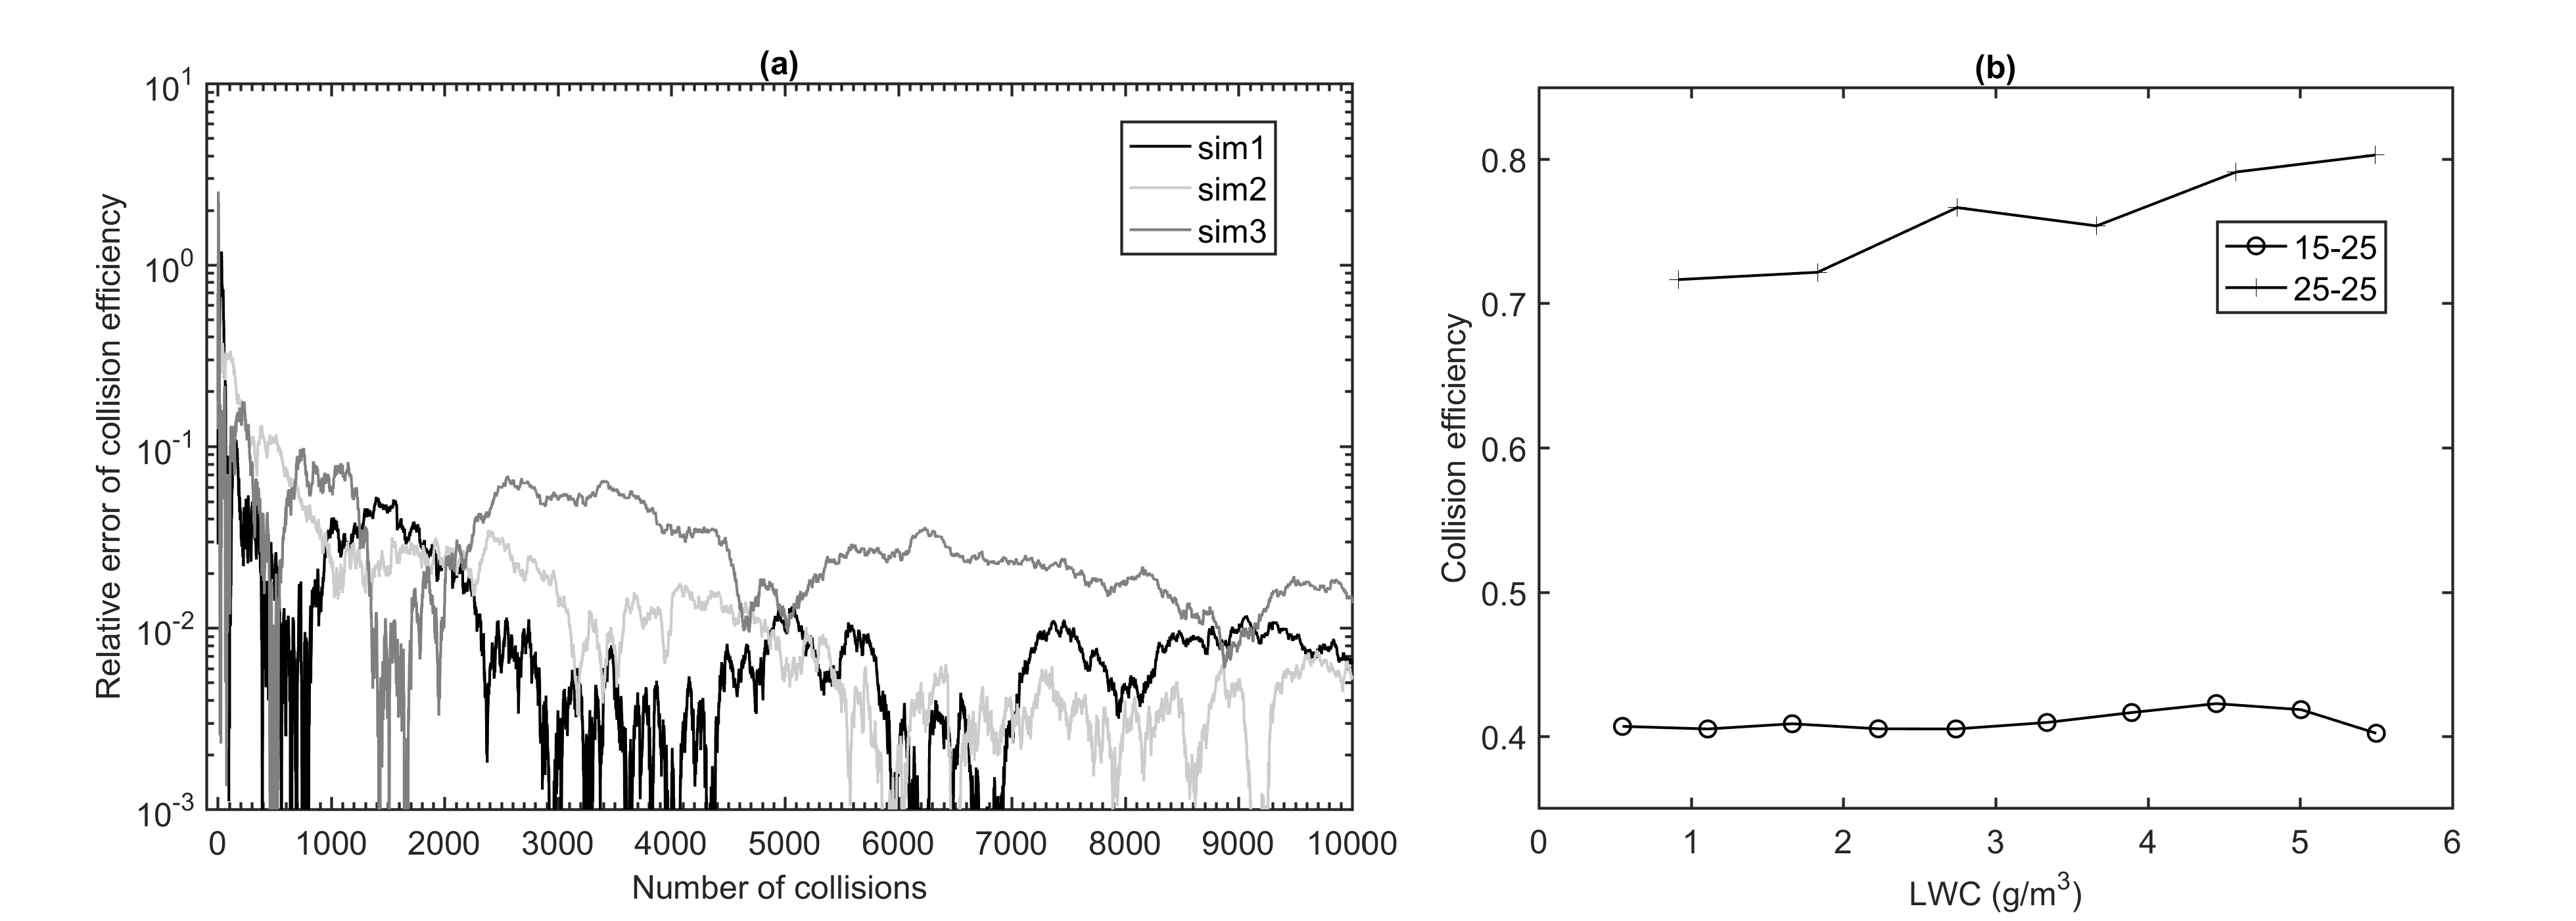
\includegraphics[width=0.8\textwidth]{Figures/Chap3/vali.png}
\caption{(a)Sensitivity test of collision efficiency on the accumulated number of collisions sampled. The $15-25$ $\mu m$ droplet pair is selected to run the simulation. Sim1, sim2, sim3 in the legend denote simulations with different initial droplet locations. (b) Dependency of collision efficiency on the liquid water content (LWC). The droplet pair of $15-25$ $\mu m$ is selected to test the cross-sized collision case and $25-25$ $\mu m$ to test the same-sized collision case. All simulations have a dissipation rate of $500 cm^2s^{-3}$.  } \label{fig:vali}
\end{figure}

The liquid water content (LWC) of all simulations is constrained between 0.1 and 6 $gm^{-3}$, which is a compromise between the droplet size, droplet number concentration, and the typical adiabatic LWCs for cumulus clouds (on the order of 1$gm^{-3}$). \citet{Wang2008} stated that for a system with multiple droplets, collision efficiency not only depends on the disturbance flows by the colliding droplets (near-field pair interaction), but also can be highly impacted by the disturbance flows of surrounding droplets in the system (far-field multi-body interaction) when the droplet mean separation distance is small (i.e., a high LWC). In particular, this impact is more significant for same-sized collisions mainly because the hydrodynamic interaction time between nearly equal-sized droplets are much longer. To investigate the importance of the far-field effect on cross-sized collisions and same-sized collisions, sensitivity tests over the range of LWC are conducted. We choose droplet pairs of 15-25 $\mu m$ for the cross-sized case and 25-25 $\mu m$ for the same-sized case. Simulations with different droplet number concentrations, corresponding to LWC from 0.5 to 5.5 $gm^{-3}$, are performed for both cases  at a dissipation rate of 500 $cm^2s^{-3}$ . The curve of the 15-25 $\mu m$ collision efficiency stays nearly constant, with fluctuations less than 5\% from the mean, showing insignificant influence by the LWCs considered (Fig. \ref{fig:vali}(b)). The same-sized collision efficiency increases slightly with LWC, which agrees with \citet{Wang2008}, but with a smaller increase. We conclude that for cross-sized collision events, far-field effects can be neglected and the collision efficiencies obtained in this study are valid and are applicable to cumulus clouds. In the meantime, caution should be exercised when interpreting same-sized collision results. The LWC values for all mono-disperse cases in this study are listed in table \ref{tab:LWC}.

\begin{table}[ht]
\def\arraystretch{1.5}
\begin{center}
\caption{LWC ($g m^{-3}$) in the monodisperse simulations\strut}\label{tab:LWC}
\begin{tabular}{cccccc}
\hline\hline
\multirow{2}{*}{Droplet size ($\mu m$)} & \multicolumn{5}{c}{$\epsilon$ ($cm^2s^{-3}$)} \\
\cline{2-6}
 & 20 & 50 & 100 & 200 & 500 \\
\hline
10 & 0.106 & 0.105 & 0.178 & 0.298 & 0.586\\
15 & 0.357 & 0.356 & 0.593 & 1.005 & 1.978 \\
20 & 0.423 & 0.844 & 1.406 & 2.383 & 1.875 \\
25 & 0.827 & 1.648 & 2.746 & 4.655 & 5.494 \\
 \hline
\end{tabular}
\end{center}
\end{table}


\section{Result and analysis} \label{sec:ch3_result}


\subsection{Collision efficiency} \label{sec:ch3_reCE}

In this section, four sizes of collector droplets ($r =$ 10, 15, 20, 25 $\mu m$) are investigated, and collision statistics of 28 droplet pair combinations at zero turbulence (Stokes flow simulations) and five turbulence intensities ($\epsilon=$20, 50, 100, 200, 500 $cm^2s^{-3}$) are analyzed. All collision efficiencies are tabulated in the appendix  as they can be applied in the stochastic collision equation or can be used to develop parameterization schemes.

Figure \ref{fig:cer_ratio} demonstrates the variation of collision efficiency with r-ratio, defined as the radius ratio of collected and collector droplet ($r_1/r_2$). For a brief comparison with previous studies, we mention that similar trends are observed among our curves and the results from \citet{Pinsky2008} and \citet{Wang2008}. In particular, our collision efficiency quantitatively agrees well with \citet{Pinsky2008} for most cases while slightly greater for $r_2=20$ $\mu m$ when $r_1/r_2 < 0.7$. However, greater values are observed in \citet{Wang2008}. This difference can be caused partially by the possible overestimation of far-field aerodynamical interaction in their case due to the high LWCs and partially by the different fluid parameters ($\nu$, $\rho_d$, $\rho_a$, etc.) chosen to calculate droplet terminal velocity. Overall, the collision efficiency shows convergence at weak turbulence and increases with dissipation rate. \citet{Wang2008} found that, for cross-sized collisions, collision efficiency exhibits a strongly positive correlation to the reduction of droplet relative velocity, due to the presence of the disturbance flow. The turbulence enhancement of collision efficiency is mainly because the disturbance flow becomes less effective in reducing the droplet relative velocity when turbulence is present. We can extrapolate that as turbulence continues to intensify, the influence of the disturbance flow diminishes and the collision kernel converges to the geometric collision kernel at a different rate for various r-ratios.  


\begin{figure}[ht]
\centering
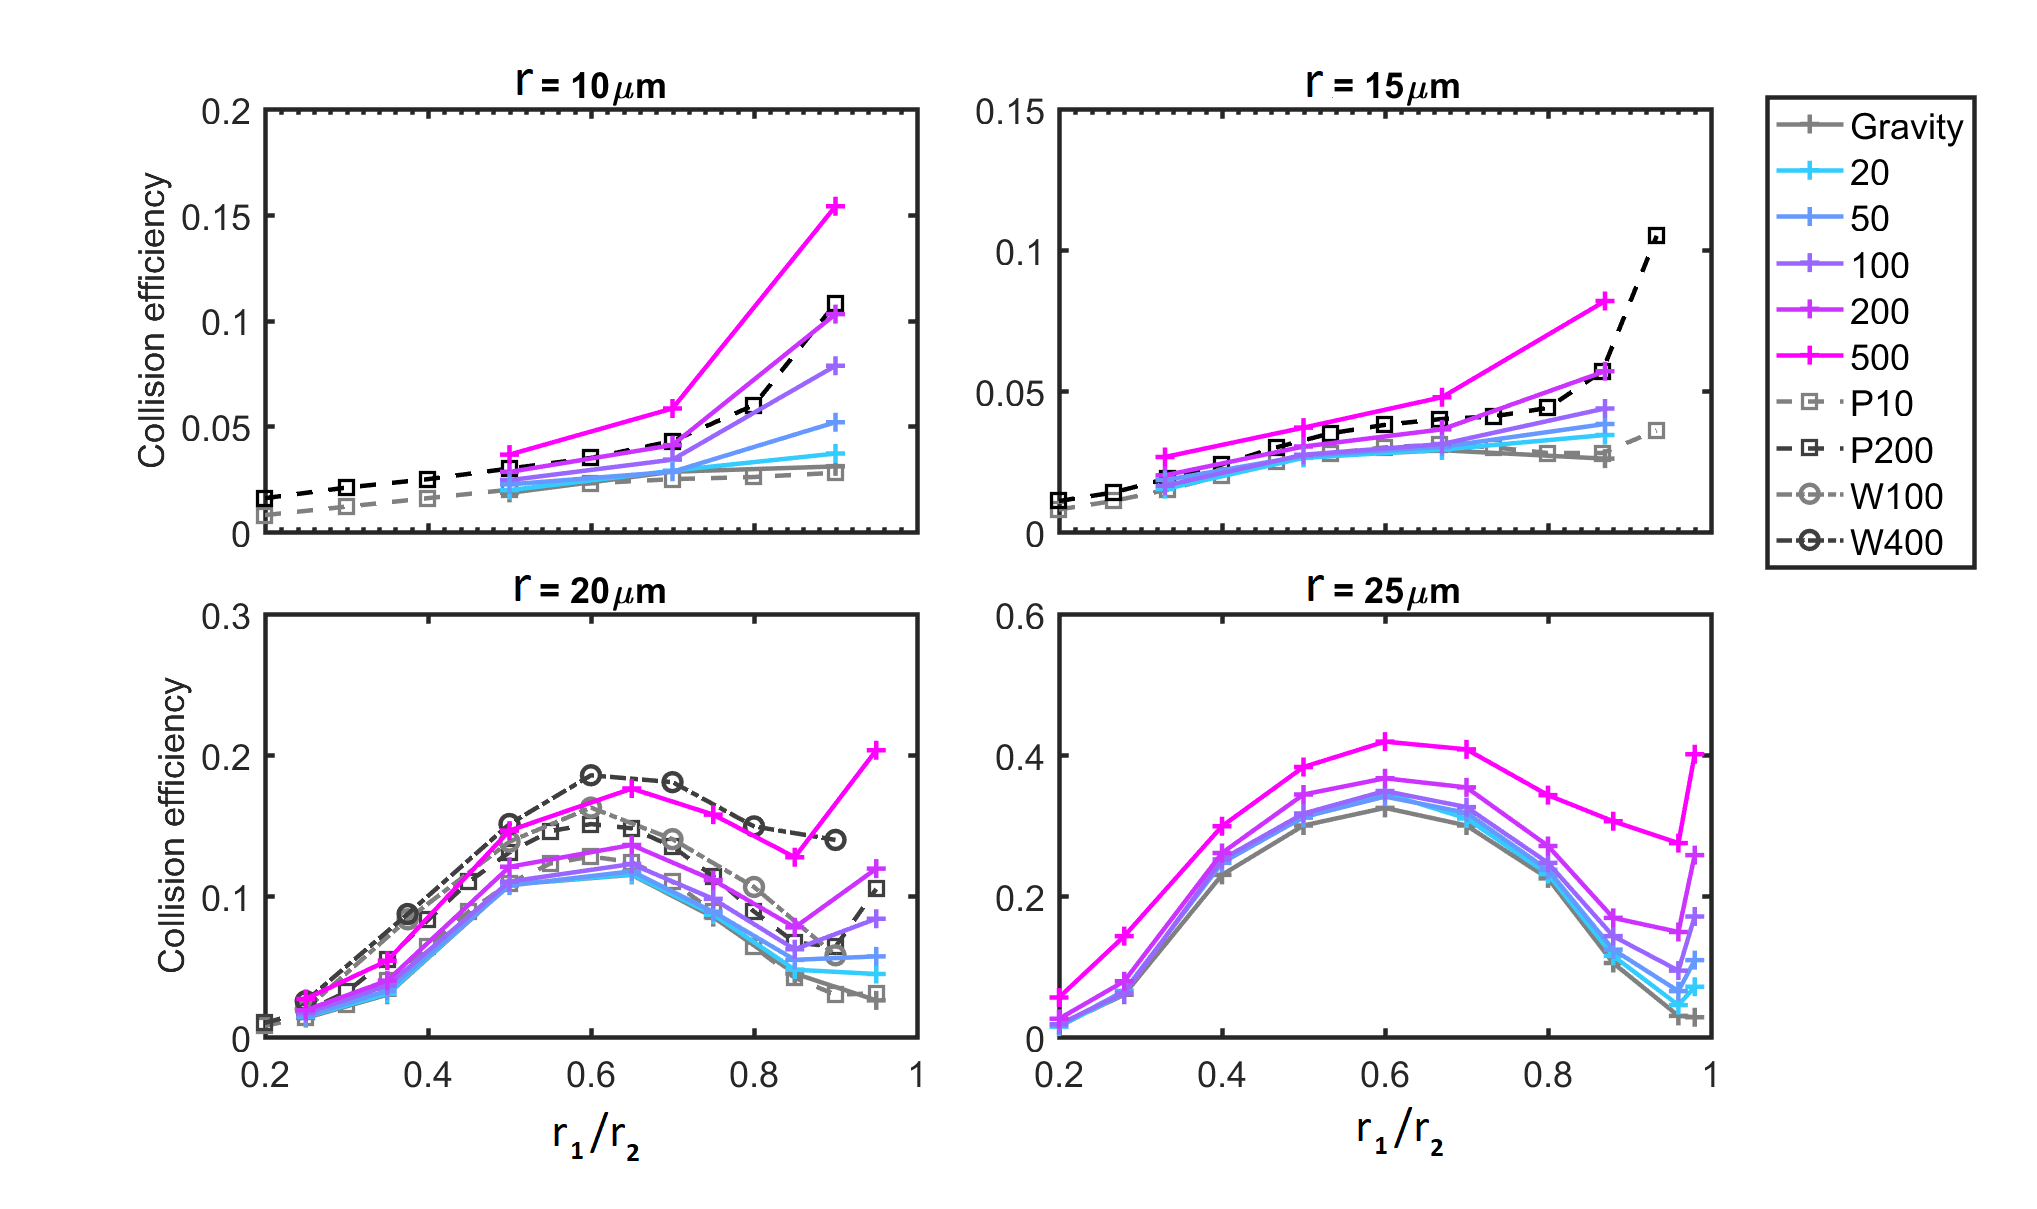
\includegraphics[width=0.8\textwidth]{Figures/Chap3/cer_ratio.png}
\caption{Collision efficiency for different collector droplets as a function of r-ratio at different turbulent environments for four different sizes of collector droplets (shown in the title of each panel). Colors demarcate dissipation rates with corresponding values  (in $cm^2s^{-3}$) shown in the legend. Collision efficiency from \citet{Pinsky2008} (dashed line with squares) and \citet{Wang2008} (dashed line with circles) are shown for comparison with dissipation rates listed in the legend. The collision efficiency of \citet{Wang2008} is produced from the multiplication of the enhancement factor from their table B.4. and gravitational collision efficiency from \citet{Wang2005a}. } \label{fig:cer_ratio}
\end{figure}

To examine how turbulence enhancement varies with r-ratio, we calculate the enhancement factor, which is defined as the collision efficiency normalized by its gravitational value. Figure \ref{fig:enhance} shows the enhancement factor of the four collector droplets at the dissipation rate of $\epsilon = 200 cm^2s^{-3}$. As can be seen, the trend is consistent with the enhancement calculated from \citet{Pinsky2008} at $\epsilon = 200 cm^2s^{-3}$ and \citet{Wang2008} at $\epsilon = 100 cm^2s^{-3}$. Enhancement is greatest for similar-sized collisions, indicating that turbulence has its strongest influence in modifying the hydrodynamic interactions between droplets of similar sizes. The enhancement is very weak and stays below 1.5 for $0.2 < r_1/r_2 < 0.8$. According to \citet{Pinsky2008} (purple dashed line in the figure), the enhancement at small r-ratio ($r_1/r_2 < 0.2$) has a comparably large magnitude with the similar-sized case, i.e., collisions containing tiny droplets. However, the collision efficiency of those minuscule droplets remains tiny even after the inclusion of the turbulence effect. This is mainly because tiny droplets tend to follow the flow due to their small inertia. Therefore, turbulence effects make their largest contribution in altering the collision rates between similar-sized droplets. Another intriguing finding is that the enhancement is highly sensitive to the r-ratio but weakly dependent on the size of collector droplets given a fixed r-ratio. This indicates a potential simplification in future parameterizations of the turbulent enhancement of collision efficiency for droplets less than 25 $\mu m$, as those sizes are crucial to initiating effective gravitational collisions. However, it is noteworthy that this feature does not hold for larger droplets. As shown by \citet{Wang2008}, the enhancement weakens as the collector droplet reach 30 $\mu m$ and beyond. 


\begin{figure}[ht]
\centering
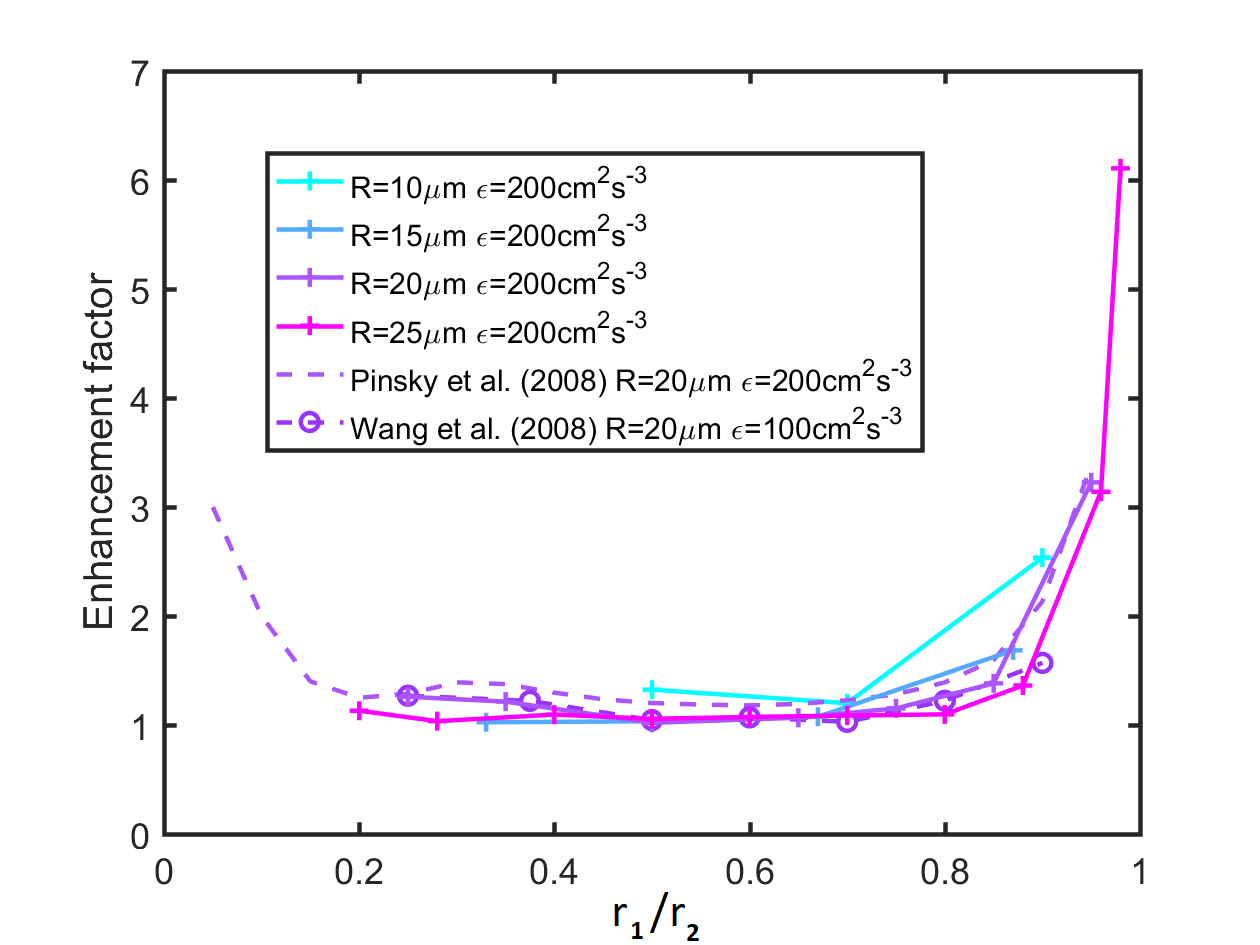
\includegraphics[width=0.8\textwidth]{Figures/Chap3/enhance.png}
\caption{ Turbulence enhancement factor of collision efficiency for all four collector droplets at dissipation rate of 200 $cm^2s^{-3}$ (shown in solid lines with cross markers). Enhancement factor of $r_2 = 20$ $\mu m$ from \citet{Wang2008} at $\epsilon = 100 cm^2s^{-3}$ with Reynolds number of 72.4 and from \citet{Pinsky2008} at $\epsilon = 200 cm^2s^{-3}$ are shown for comparison.} \label{fig:enhance}
\end{figure}


The same-sized collision efficiency remains close to unity but decreases slightly with dissipation rate (Fig. \ref{fig:samesize}(a) ). This has also been reported by \citet{Wang2008} in some cases. However no conclusive explanation was given due to the high uncertainty in their data. A possible explanation for the decrease can be found by studying the statistics of the radial relative velocity (RRV) and the radial distribution function (RDF), owing to the fact that the disturbance flow affects collision efficiency mainly by influencing the droplet relative motion and altering the droplet clustering within its effective range. RRV is the radial component of the relative velocity of colliding droplets. Its mean value is calculated via $\langle |\mathbf{W}_r | \rangle = \left\langle \left| \mathbf{W} \cdot \frac{\mathbf{d}}{|\mathbf{d}|} \right| \right\rangle $ with $\mathbf{W}$ being the droplet relative velocity and $\mathbf{d}$ being the separation vector. RDF measures the droplet clustering and is defined by $g(R)=\frac{N_p \Omega}{V_s N_t N_1 N_2}$. $N_p$ is the number of droplet pairs at contact found in the shell of collision sphere within $N_t$ time steps. The shell volume $V_s=\frac{4\pi}{3} [(1.01\times R)^3-R^3]$ has an outer radius slightly larger than the sum of droplet radii for sufficient sampling at finite $N_t$, which is safe to do so as long as the outer radius is smaller than $1.1 \times R$ \citep{Wang2000}. Because the non-overlapping treatment alters the mean RRV and the symmetry of the droplet radial distribution at contact, corrections for both RRV and RDF should be included to achieve the correct kinematic properties \citep{Wang2005b}, i.e., $\langle |\mathbf{W}_r|\rangle^{cor}=\langle|\mathbf{W}_r |\rangle \times C_w$, and $g(R)^{corr}=g(R)\times C_g$. $C_w$ and $C_g$ are determined by the shell thickness of the collision sphere and their expressions are provided in \citet{Wang2005b}.

Figure \ref{fig:samesize}(b) displays the normalized mean RRV of four same-sized droplet pairs varying with dissipation rates. The normalization is made by taking the ratio of RRV in the DF case and the corresponding value in the nonDF case. Similar to the collision efficiency curves in panel (a), RRV also demonstrates a decaying trend with intensifying turbulence. A weak decay is also found in the normalized RDF (panel (c) in Fig. \ref{fig:samesize}), consistent with panel (a) and (b) in spite of the larger fluctuations compared to the former two statistics. It seems that the turbulence effect in counteracting the droplet disturbance flow weakens as the turbulence intensifies, regardless of the fact that the RRVs and RDFs in both DF and NonDF runs increase with eddy dissipation rate (not shown). 

\begin{figure}[ht]
\centering
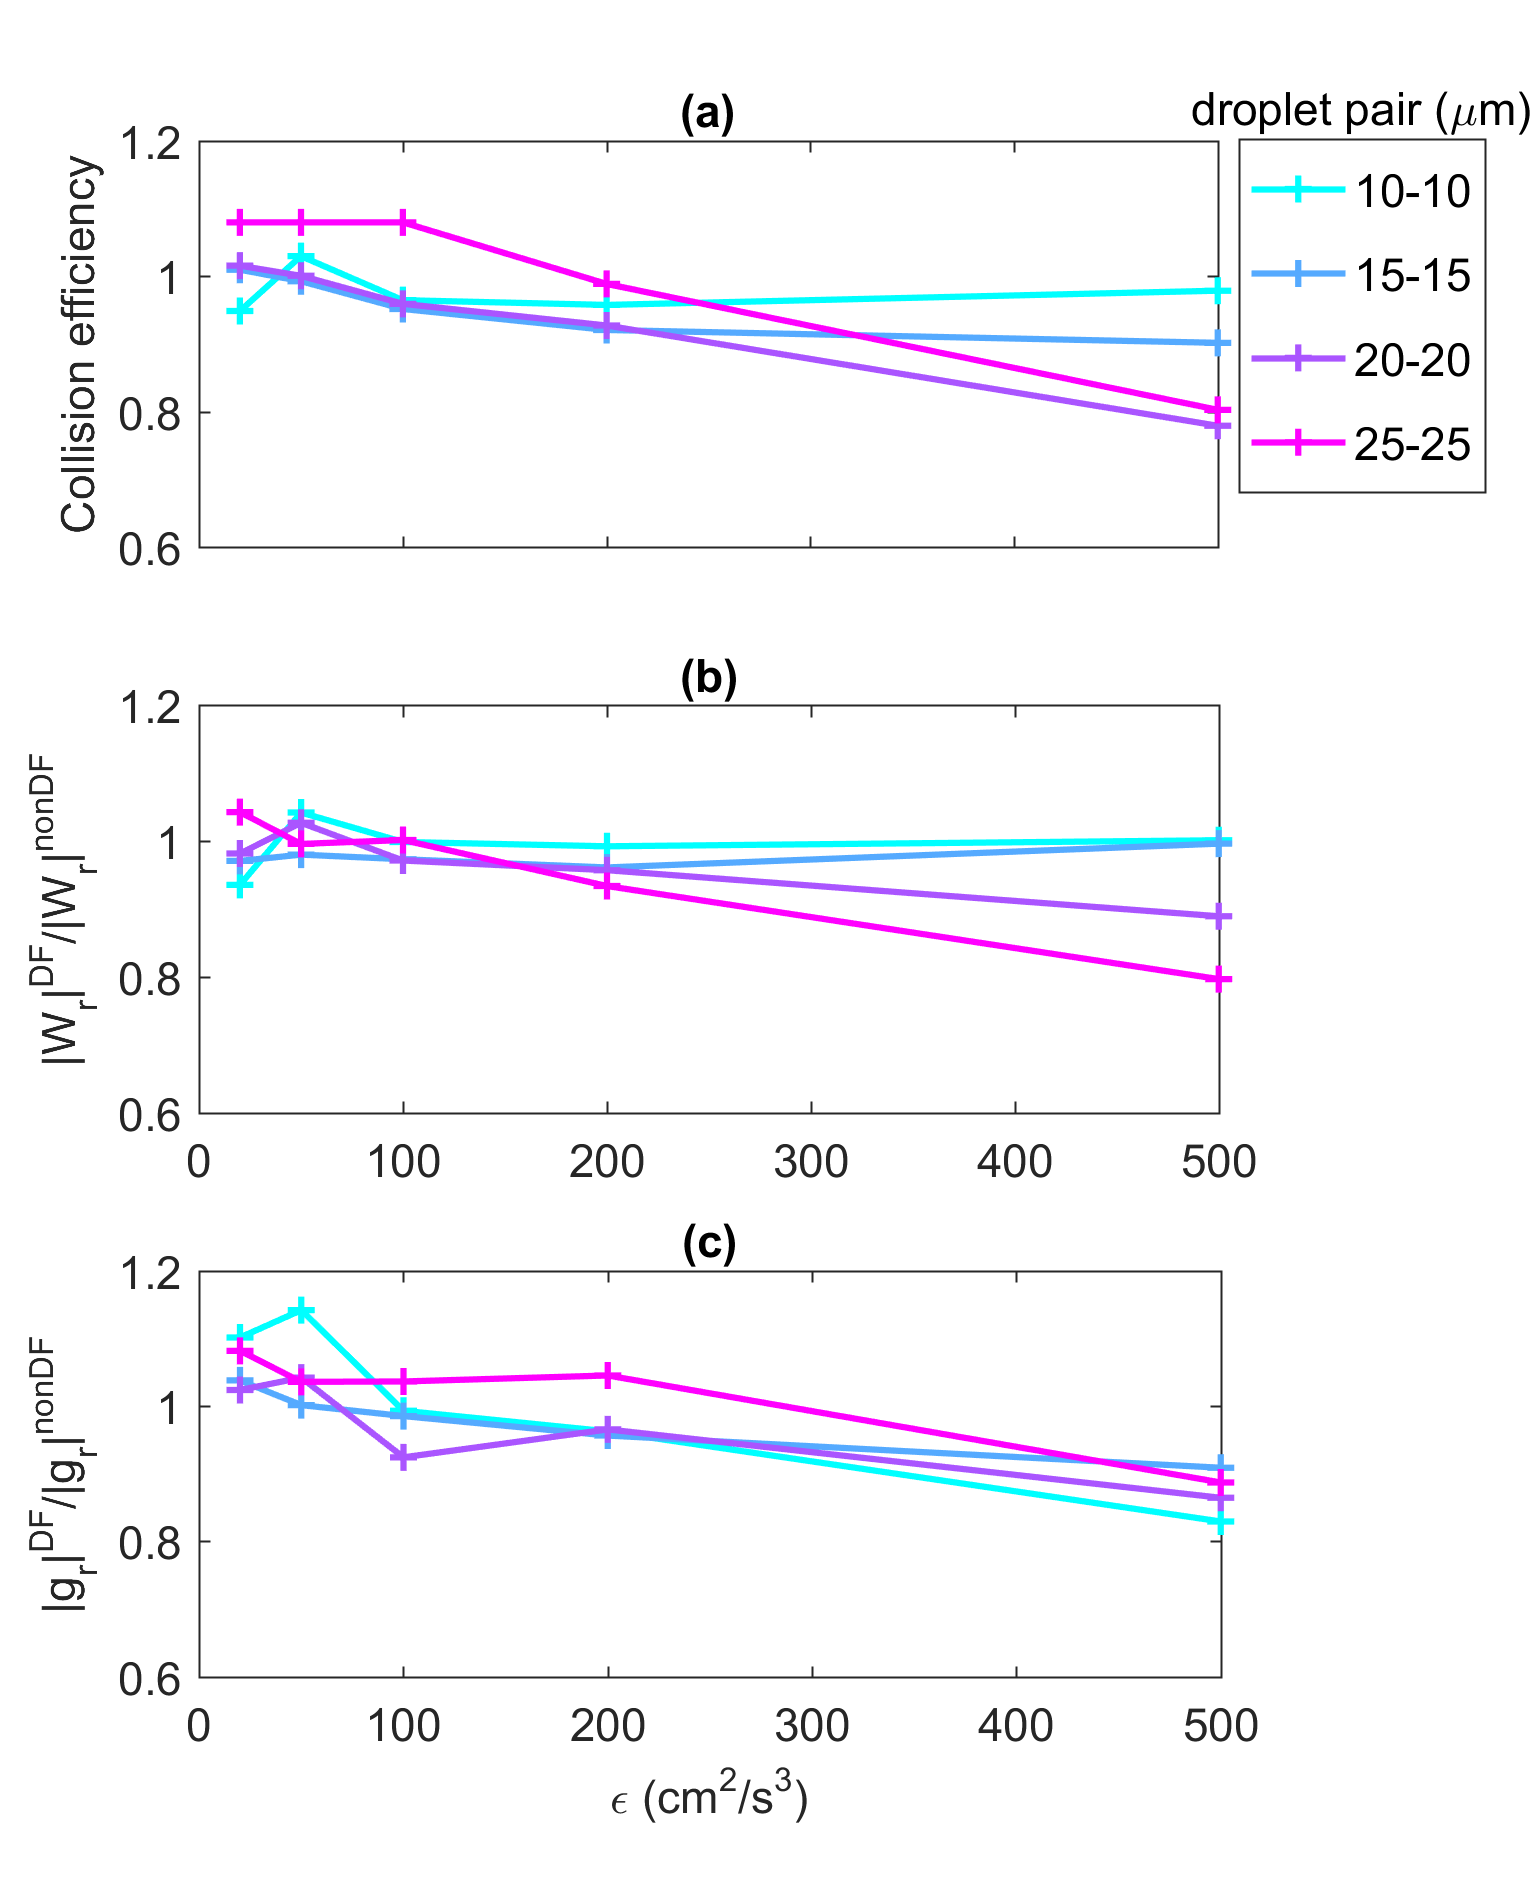
\includegraphics[width=0.8\textwidth]{Figures/Chap3/samesize.png}
\caption{Same-sized collision statistics of (a) Collision efficiency, (b) Normalized radial relative velocity in DF case by nonDF case, and (c) normalized radial distribution function as function of dissipation rate for four different droplet sizes. The normalization in panel (b) (panel (c)) is made by taking the ratio of RRV (RDF) in the DF case and the corresponding value in the nonDF cases. } \label{fig:samesize}
\end{figure}


\subsection{Turbulent collision kernel} \label{sec:ch3_reTCK}

The turbulence enhancement of the geometric collision kernel is relatively weak in a mildly turbulent environment \citep{Ayala2008a, Chen2016}. As Fig. \ref{fig:tgck} shows, the geometric collision kernel at all turbulence intensities peaks at intermediate r-ratios and drops to its lowest at same-sized collisions. However, after taking into account the collision efficiency, the curves display a very different pattern (Fig. \ref{fig:tck}) and a significant enhancement of the collision kernel in similar-sized collisions is observed. Even though the same-sized droplet pairs have much smaller geometric collision kernels (Fig. \ref{fig:tgck}), their high collision efficiency in mild to strong turbulence moves the collision kernel to a comparable magnitude as in the intermediate r-ratio regime. For small collector droplets ($r_2 = 10$ $\mu m$), the peak at r-ratio$\sim 0.6$ disappears and the collision kernel maximizes at similar-sized droplet pairs when $\epsilon > 100$ $cm^2s^{-3}$, in agreement with \citet{Pinsky2008} (see the black dashed line in the first panel of Fig. \ref{fig:tgck}). As shown in Chapter \ref{sec:ch2}, turbulence causes a very pronounced enhancement of the local clustering and relative motion in similar-sized droplet pairs, and thus greatly increases their geometric collision kernel. In this paper, we find that the turbulence enhancement of the collision efficiency is also most intense for comparable-sized pairs. The above two factors consolidate a much stronger enhancement of collision kernel for similar-size pairs. The implication is that, as the condensational growth rate slows down as droplets get larger and concurrently narrows the size spectra, turbulence can boost the broadening process through efficient similar-sized collisions and accelerate the collisional growth.

\begin{figure}[ht]
\centering
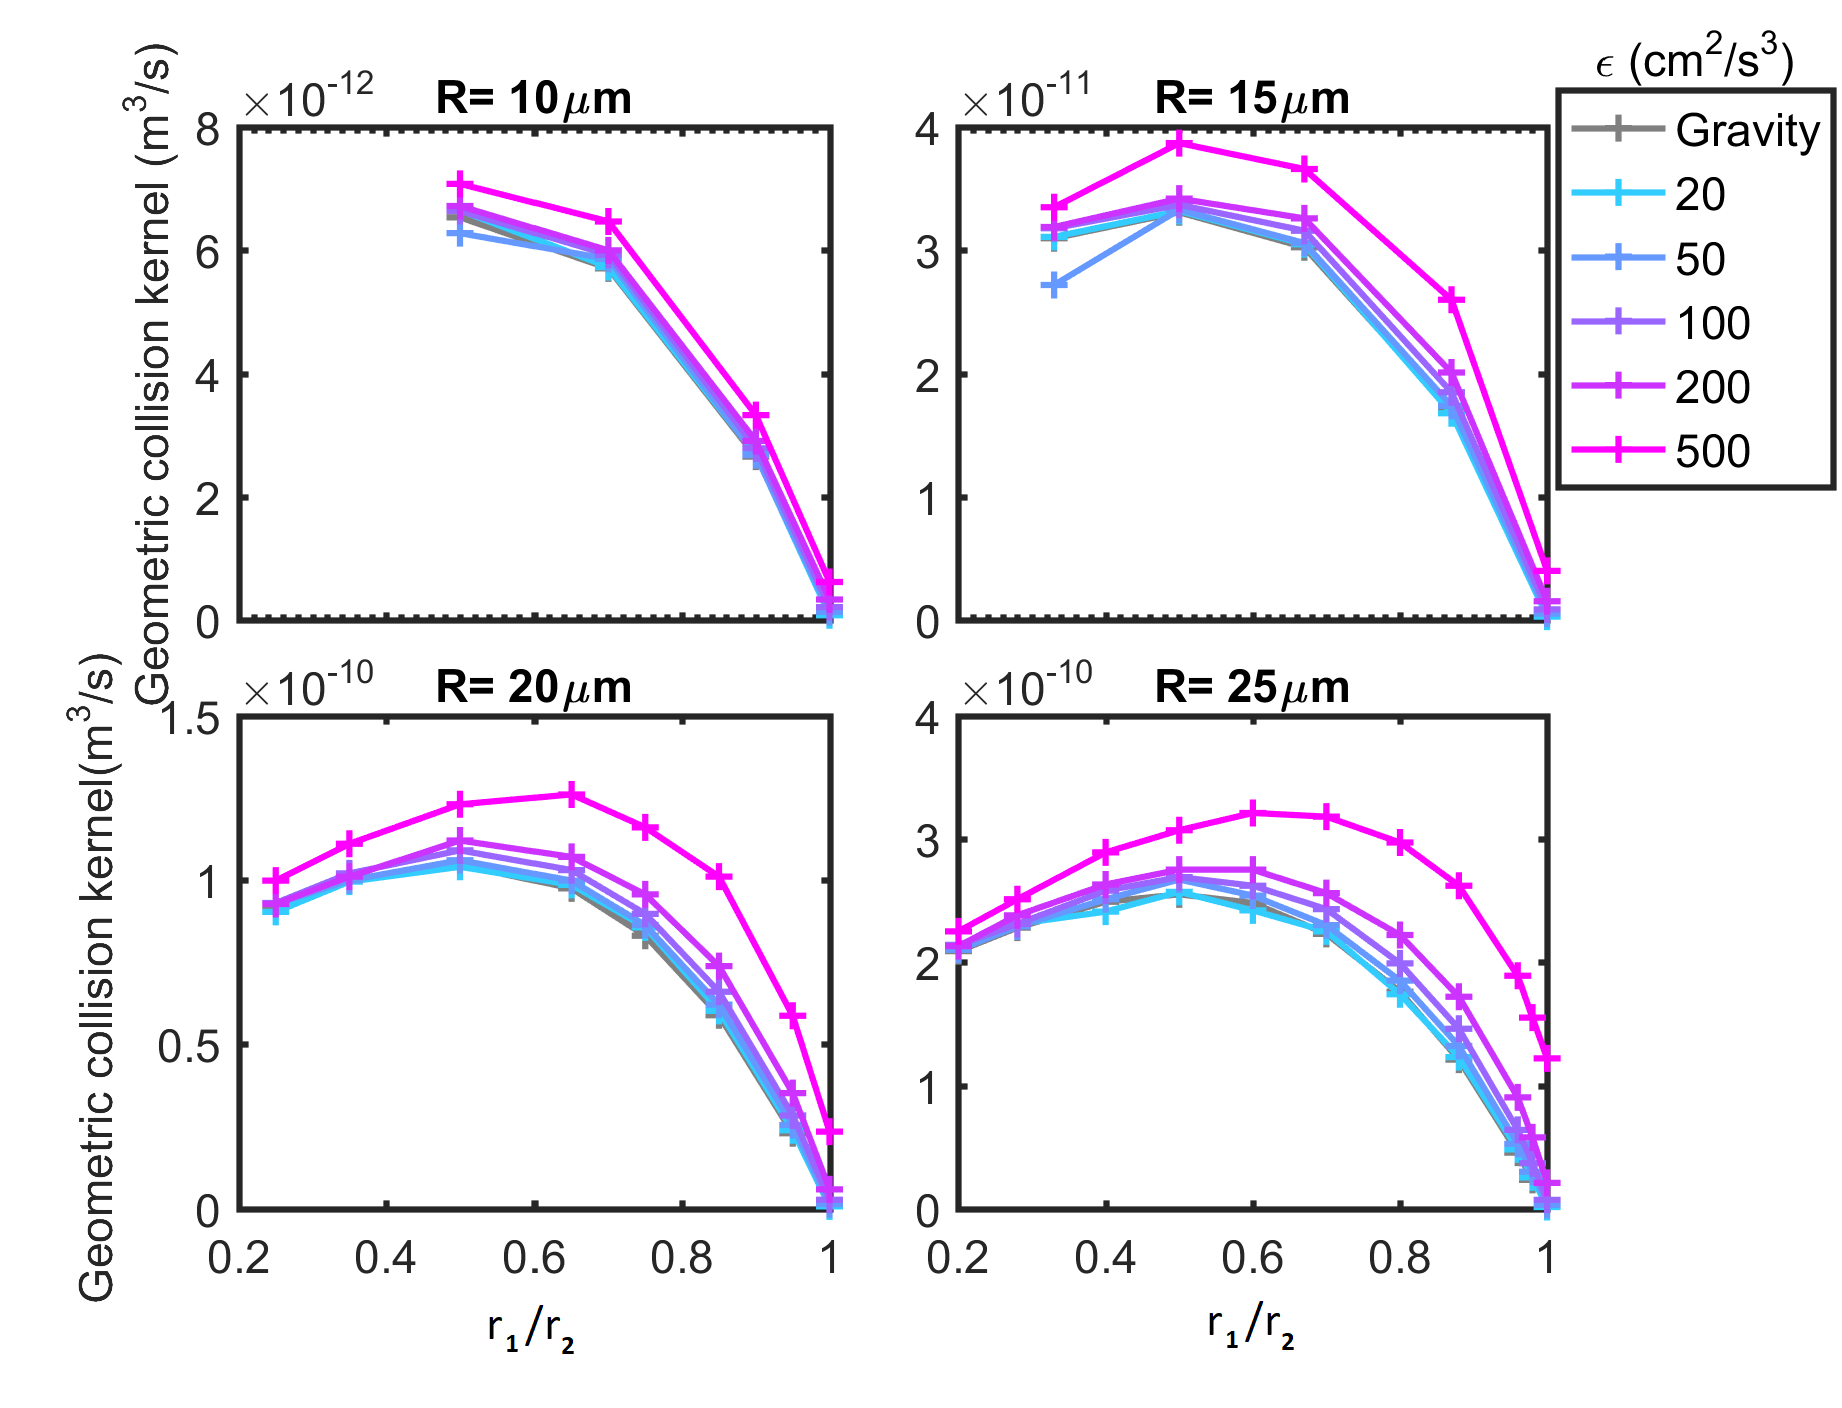
\includegraphics[width=0.8\textwidth]{Figures/Chap3/tgck.png}
\caption{Same as Fig. \ref{fig:cer_ratio} but for the turbulent geometric collision kernel ($m^3s^{-1}$).} \label{fig:tgck}
\end{figure}

\begin{figure}[ht]
\centering
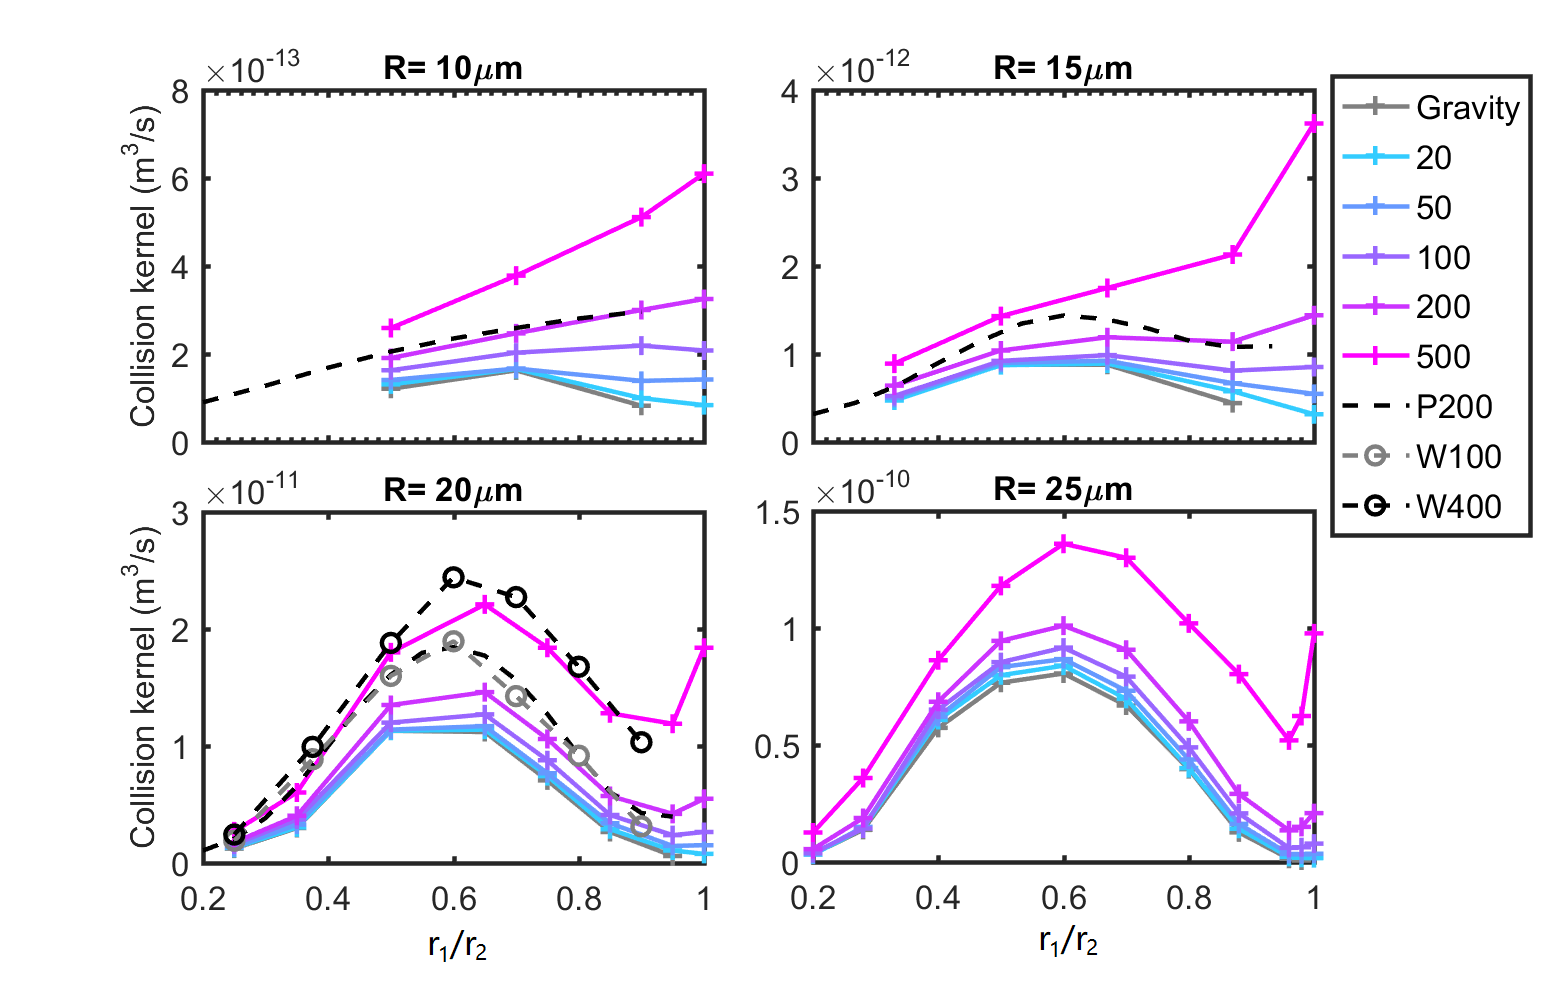
\includegraphics[width=0.8\textwidth]{Figures/Chap3/tCK.png}
\caption{same as Fig. \ref{fig:cer_ratio} but for the turbulent collision kernel ($m^3s^{-1}$). Collision kernel of $r_2 = 20$ $\mu m$ from \citet{Wang2008} at $\epsilon=100$ $cm^2s^{-3}$ and $\epsilon=400$ $cm^2s^{-3}$ with Reynolds number of 72.4 (dashed lines marked with circles and labeled as "W100" and "W400" in the legend) and from \citet{Pinsky2008} with $\epsilon=200$ $cm^2s^{-3}$ are shown for comparison (dashed lines labeled with "P200"). Dissipation rates are listed in the legend.} \label{fig:tck}
\end{figure}

\subsection{Evolution of droplet size distribution} \label{sec:ch3_reDSD}

To illustrate the turbulence broadening hypothesis in the last section, we conduct simulations that allow droplets to grow by collision-coalescence to investigate the impact of turbulence on DSD evolution. 

The initial shape of DSD (green dashed lines in Fig. \ref{fig:DSD}) is adopted from an aircraft observation through cumulus clouds off the coast of Hawaii \citep{Raga1990}. LWC is fixed at a typical adiabatic value of 1 $gm^{-3}$. Four dissipation rates are investigated ($\epsilon$ = 50, 100, 200, and 500 $cm^2s^{-3}$) and this range covers the most frequently observed turbulent environments observed in cumulus and stratocumulus clouds. A simulation without turbulence will also be performed for comparison. We run each simulation for 6.5 minutes of real time and observe the time evolution of the DSD. To reduce the impact of initial conditions in the pure-gravity case, three ensemble runs with different initial droplet locations are performed, and the mean value of the three realizations is used in the analysis.

Figure \ref{fig:DSD} depicts the droplet size spectra and mass density spectra at the end of the simulations. The discontinuous tails of the distributions result from the few large droplets formed in the domain. While broadening of the spectrum in the form of an exponential tail occurs in all experiments, the broadest spectrum is observed at our strongest turbulence. The number and mass of large droplets ($r > 20$ $\mu m$) for the gravity case stays lowest among the five simulations. Figure \ref{fig:timeDSD} shows the DSD evolution of the same five simulations. Droplet number concentrations below 0.001 $cm^{-3}$ are treated as statistical uncertainty since they correspond to less than 2-3 droplets in the domain, and thus there is no color in the plot. As expected, the DSD of the pure gravitational case stays relatively narrow throughout the simulation (panel (a) of Fig. \ref{fig:timeDSD}).) and droplets larger than 30 $\mu$m remain "invisible". In comparison, droplets grow larger than 35 $\mu$m at the end of all simulations with turbulence(see the purple colored edge in \ref{fig:timeDSD}). This again indicates that even weak turbulence plays an efficient role in DSD broadening and produces a considerable number of large droplets. As dissipation rate continues to increase, the distribution tail expands at a faster pace. In the case with $\epsilon=500$ $cm^2s^{-3}$, droplets larger than 45 $\mu$m can be visible at the end and the largest droplet reaches 68 $\mu$m. 

\begin{figure}[ht]
\centering
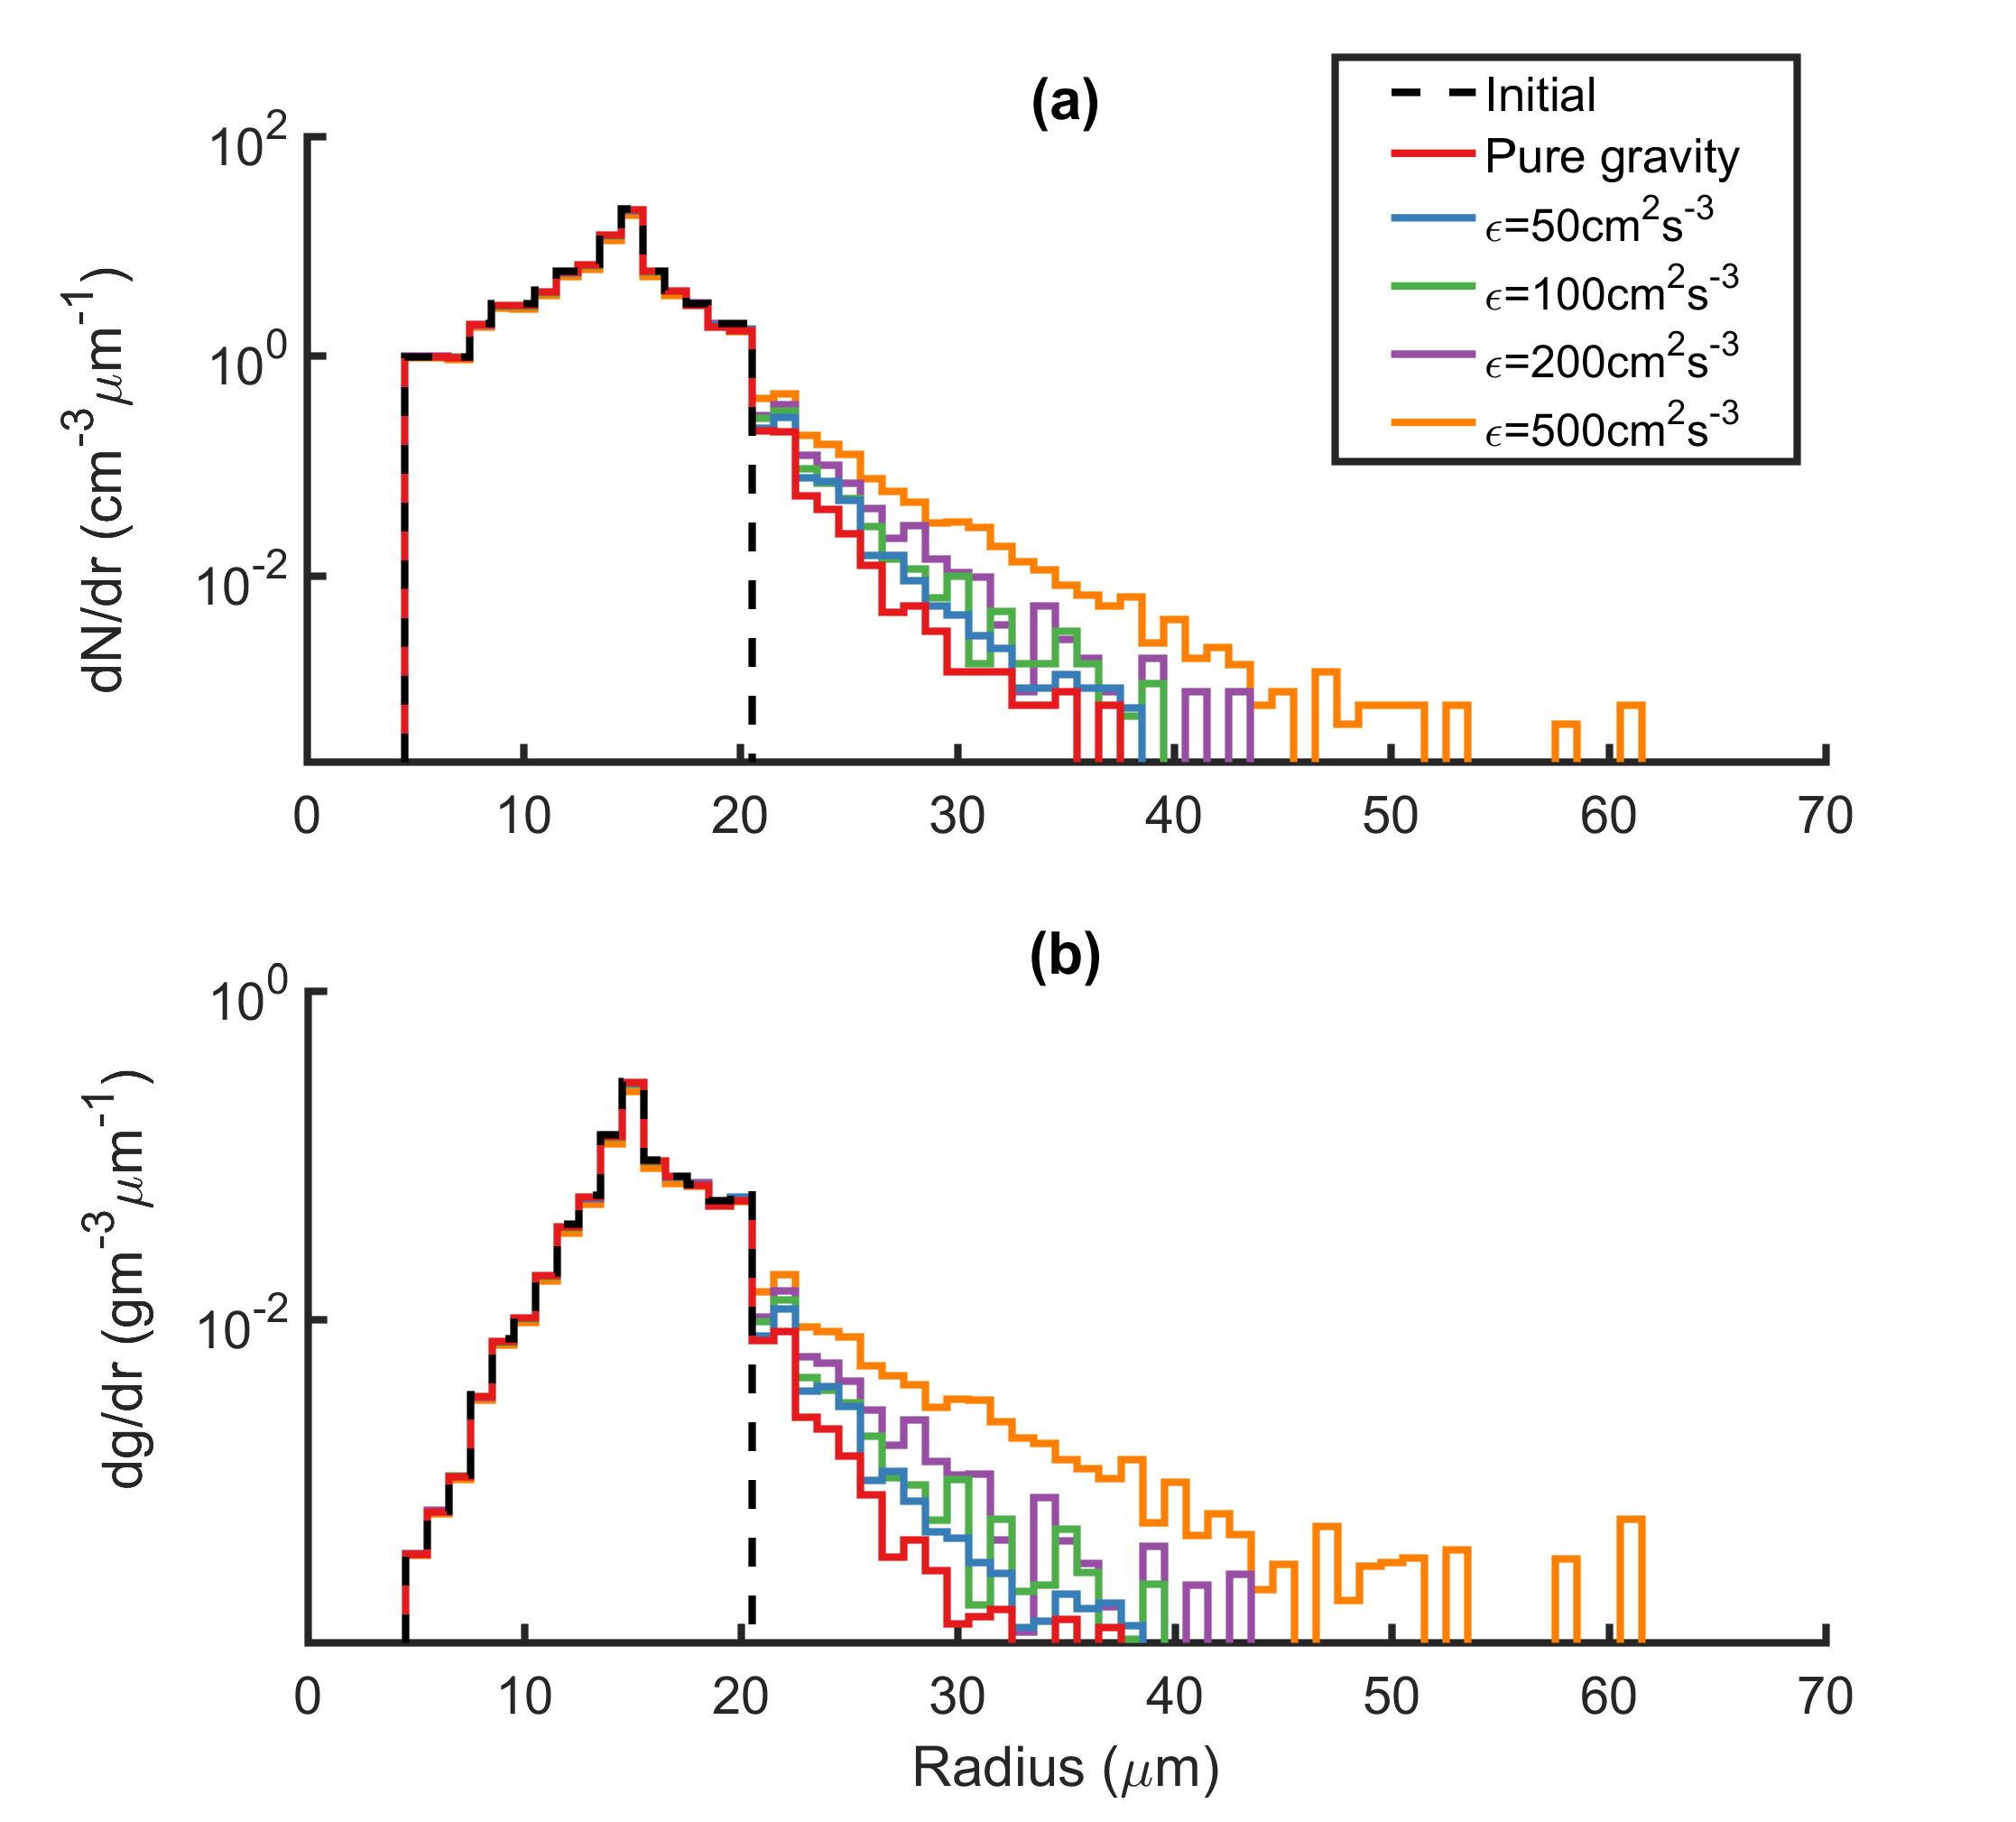
\includegraphics[width=0.8\textwidth]{Figures/Chap3/DSD.png}
\caption{(a) Droplet size distribution and (b) mass density distribution at the 6.5th minute in five different turbulence environments ($\epsilon=0, 50, 100, 200, 500$ $cm^2 s^{-3}$). The initial DSD (black dashed line) is adopted from the flight observation \citet{Raga1990}. LWC is kept 1 $g/m^3$ for all simulations.} \label{fig:DSD}
\end{figure}

\begin{figure}[ht]
\centering
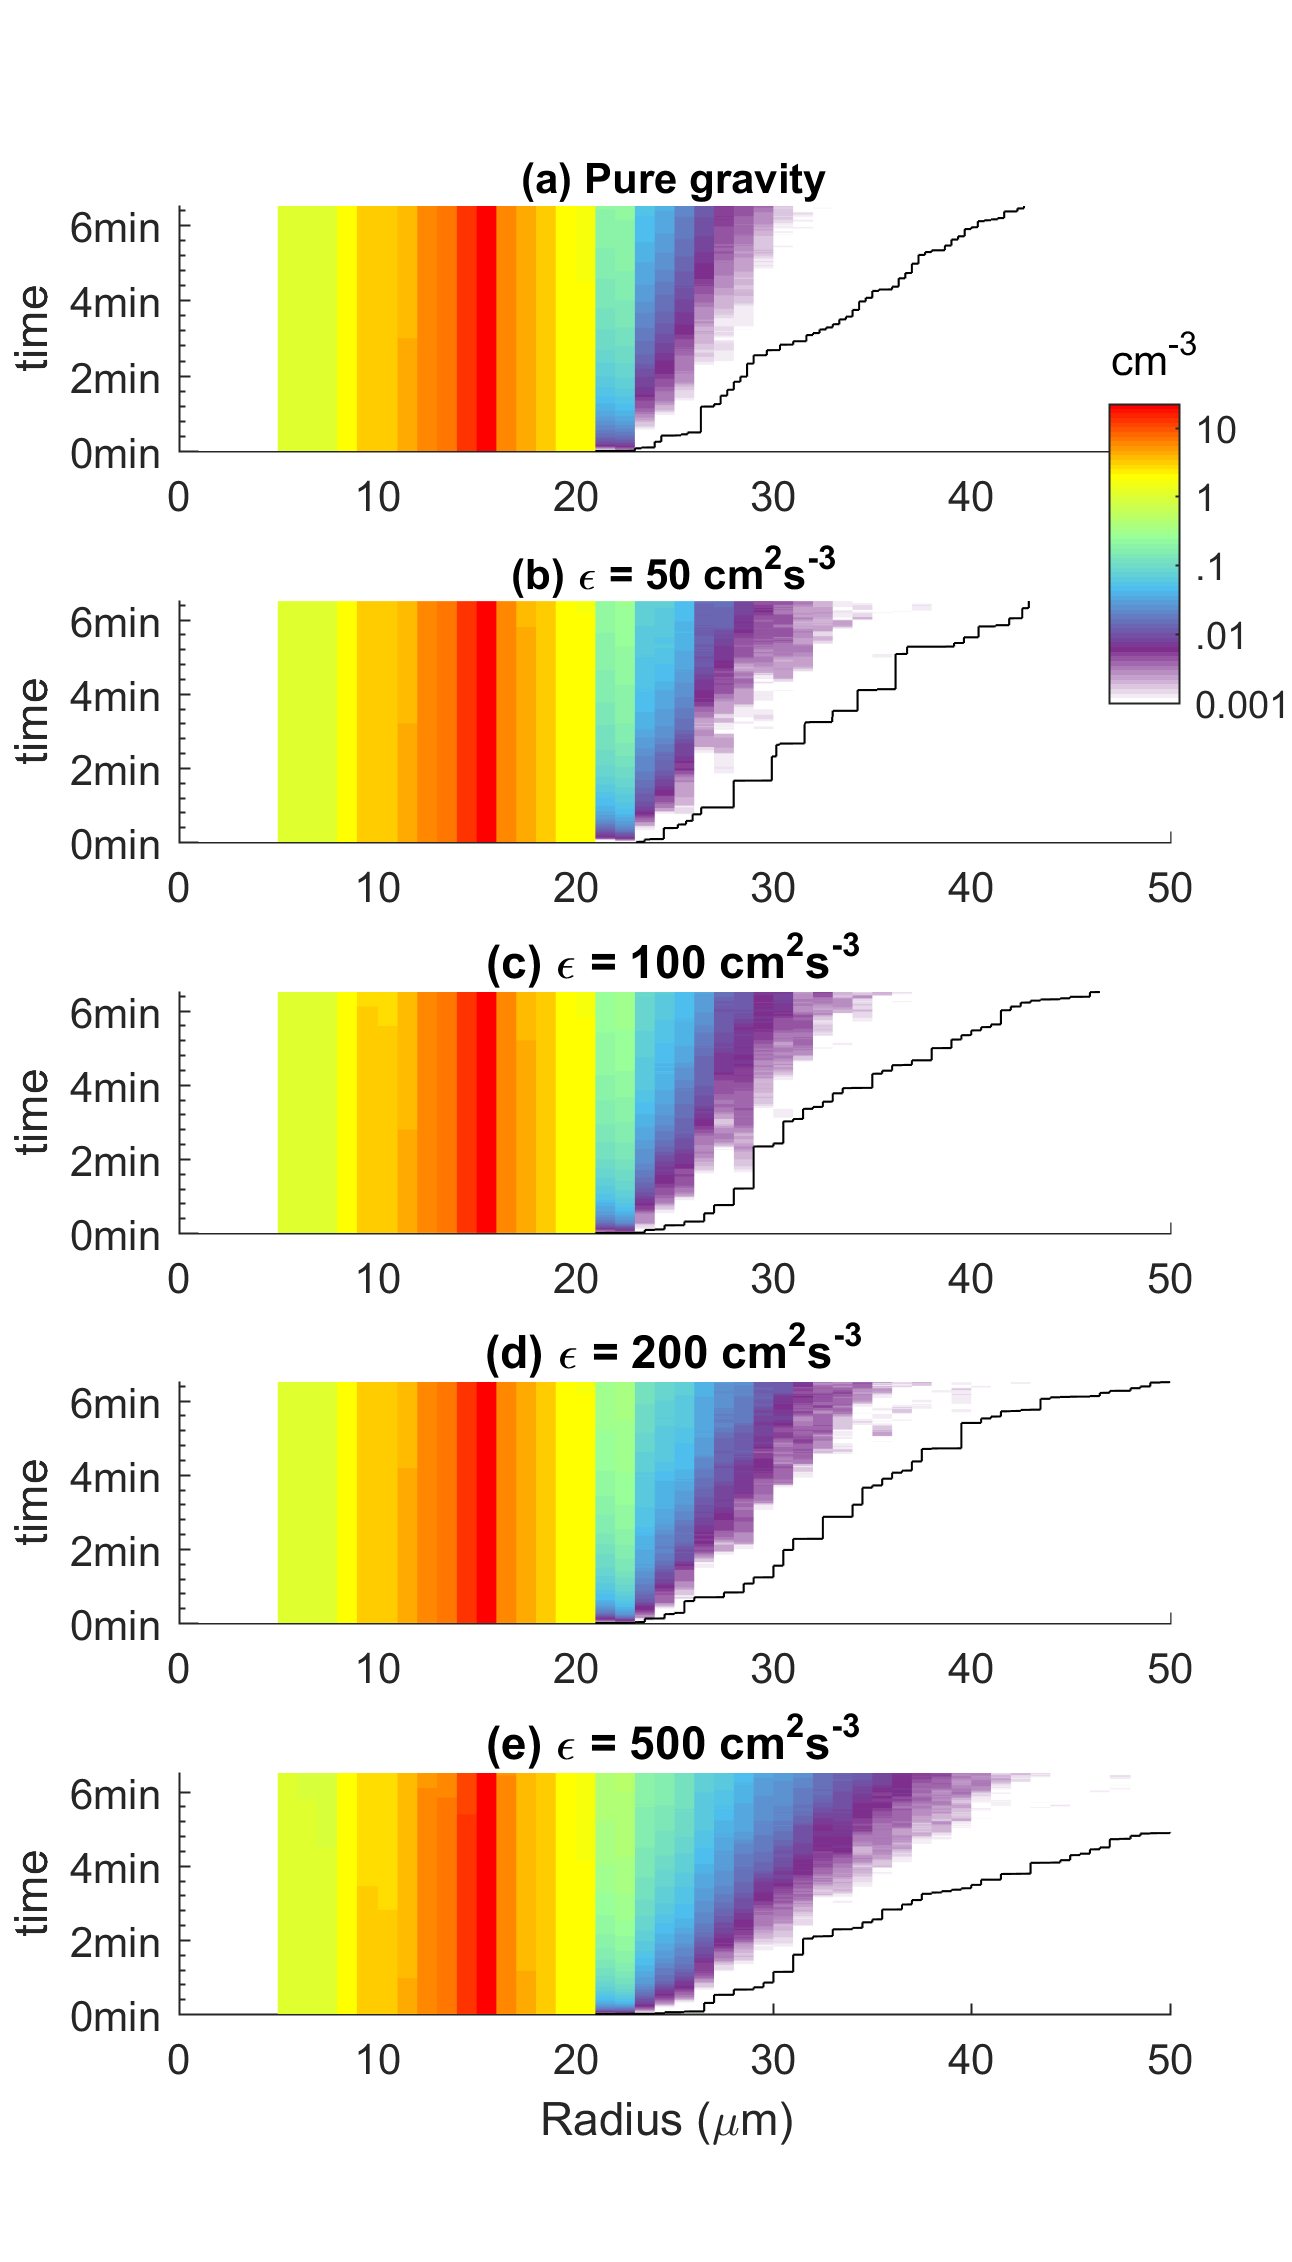
\includegraphics[width=0.5\textwidth]{Figures/Chap3/timeDSD.png}
\caption{: Evolution of droplet size spectra from the same four simulations as described in Fig \ref{fig:DSD}. The color demarcates different number concentrations of each droplet-size bin, with white mapping the concentration below 0.001 $cm^{-3}$. The black curve indicates the size of the largest droplet that occurs in the simulation.} \label{fig:timeDSD}
\end{figure}


To evaluate the collision contribution to the DSD evolution from different r-ratios, we calculate the average collision frequency during the simulation for droplet pairs in various r-ratio bins (Fig. \ref{fig:freq}). As turbulence intensifies, a considerably higher collision frequency is observed from all size groups. Particularly, the largest increment comes from similar-sized collisions. At the pure gravity case, most collisions are from $r_1/r_2\in(0.6,0.8)$. When turbulence gets stronger, the collision frequency distribution becomes heavily skewed. In the simulation of dissipation rate 500 $cm^2s^{-3}$ the number of collisions with $r/r_2>0.9$ increases by more than a factor of 10 compared to the gravitational case, while the enhancement factor of collisions from $r_1/r_2\in(0.6,0.8)$ is smaller than 4. Table \ref{tab:collision} lists the contribution of collisions (probability density function) from different r-ratio ranges. In turbulent cases, similar-sized collisions ($r_1/r_2 > 0.8$) alone account for nearly a quarter of the total collisions. In contrast, only 9.36\% of the collisions are from similar-sized collisions in the gravitational case. In other words, the enhanced broadening by turbulence is largely coming from similar-sized droplet collisions, and even a weak turbulent environment can boost those collisions. However it should be noted that the superposition method does not treat the lubrication effect adequately \citep{Rosa2011,Wang2005a}, and thus the likely overestimation of collision efficiency may lead to faster droplet growth in both the pure-gravity case and the turbulent case.
 

\begin{figure}[ht]
\centering
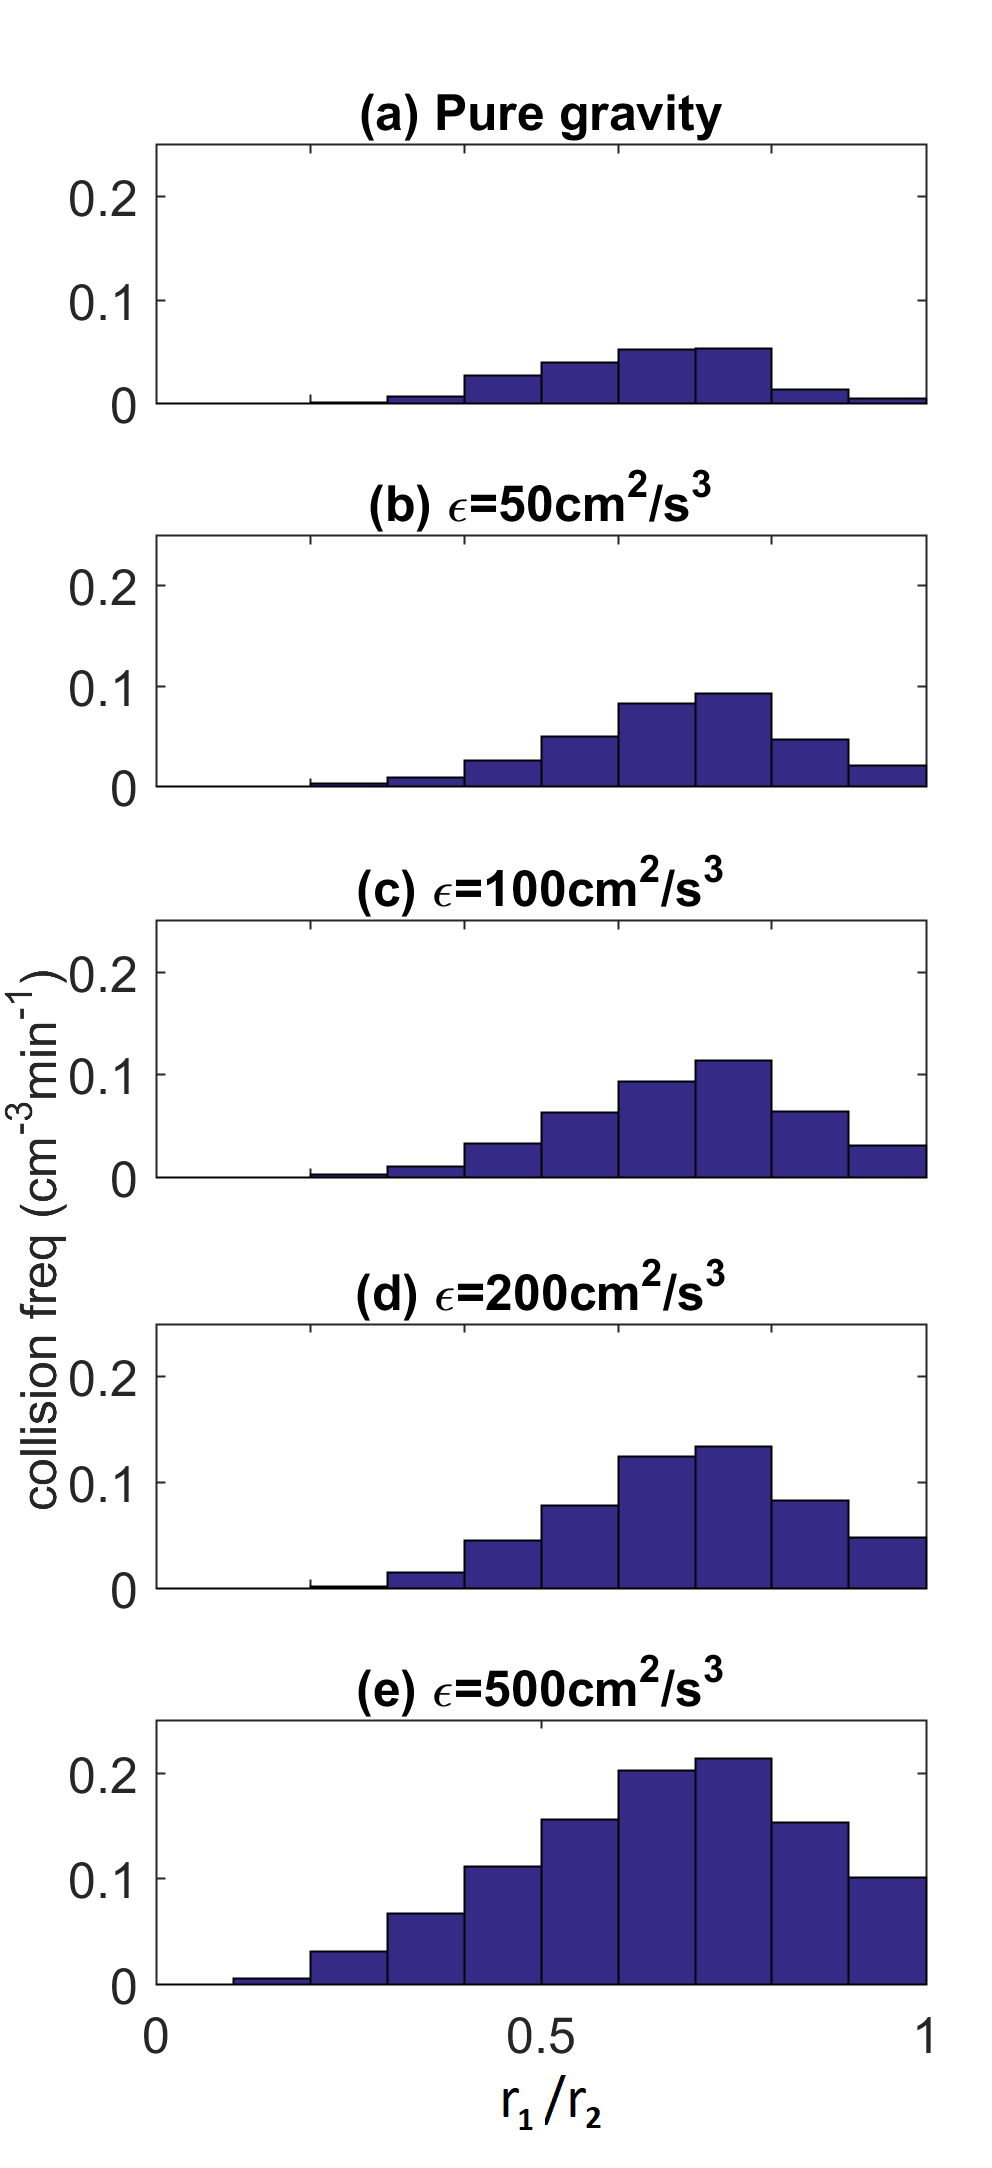
\includegraphics[width=0.4\textwidth]{Figures/Chap3/freq.png}
\caption{Frequency distribution of collisions from different droplet size groups (i.e., different r-ratios) from the four different turbulence environments. The collision frequency is defined as the average number of collisions occurring in each r-ratio bin in unit time ($min ^{-1}$) and in unit volume ($cm^{-3}$) during the entire 6.5 min simulation. The r-ratio is equally divided into ten bins with 0.1 of width for each bin.} \label{fig:freq}
\end{figure}

\begin{table}[ht]
\begin{center}
\caption{contributions (\%) of collisions from different r-ratio ranges in four turbulent cases during 6.5 min simulation.\strut}\label{tab:collision}
\begin{tabular}{c|ccccc}
\hline\hline
\backslashbox{$r_1/r_2$}{$\epsilon$ ($cm^2s^{-3}$)} & 0 & 50 & 100 & 200 & 500 \\
\hline
(0,0.3] & 0.65\% & 1.09\% & 0.53\% & 0.38\% & 3.54\%\\
(0.3,0.8] & 89.99\% & 78.38\% & 76.24\% & 74.89\% & 72.08\% \\
 (0.8,1] & 9.36\% & 20.53\% & 23.23\% & 24.72\% & 24.38\% \\
  \hline
\end{tabular}
\end{center}
\end{table}


\section{Summary and outlook} \label{sec:ch3_conclusion}

The purpose of this study is to investigate and quantify the turbulence enhancement of collision efficiency as part of our continued exploration of turbulence effects on droplet growth. DNS simulations are performed to obtain turbulent collision statistics from 28 droplet-size combinations. LWC is kept at the order of typical adiabatic values to ensure that the hydrodynamic interaction between droplets possibly affected by droplet separation distance (far-field effect) well represents the typical situation in cumulus clouds. Sensitivity tests show little dependency of collision efficiency on LWC values used in this study, suggesting that far-field effects of the disturbance flow have a secondary influence. 

Five dissipation rates spanning a typical range in cumulus clouds ($\epsilon = 20-500$ $cm^2s^{-3}$) are considered, and the pure gravitational case is conducted as a control run. Overall, the turbulence effect of collision efficiency is strongly influenced by the r-ratio. In particular, similar-sized collisions experience the most pronounced enhancement. Previous studies found that turbulent enhancement of the geometric collision kernel is also strongest at similar-sized collisions (r-ratio $\rightarrow$ 1). The joint turbulence effects consolidate a significant increase of the collision kernel between similar-sized droplets. This implies that turbulence can be an effective mechanism to broaden the narrow droplet size distribution resulting from the condensational-growth stage. In addition, we find that for the droplet sizes considered, the enhancement shows little dependency on the size of collector droplet if the r-ratio is fixed. This may simplify the future parameterization as only one size parameter (r-ratio) needs to be considered for those droplet sizes. 


To further illustrate the DSD broadening process and monitor the appearance of large droplets in the early rain formation stage, this study conducts the first direct simulation of the droplet growth by collision-coalescence in the disturbed turbulence flow. The pure-gravity case along with four turbulence intensities ($\epsilon = 50-500$ $cm^2s^{-3}$) are examined with the same initial DSD adopted from aircraft observations of cumulus clouds. While DSD broadening is observed in all simulations, the broadest spectrum occurs in our strongest turbulence. In comparison to the gravitational case, where the DSD stays narrow and droplets hardly exceed 30 $\mu$m throughout the simulation, droplets larger than 35 $\mu$m are seen in all turbulence simulations. In the meantime, similar-sized collisions account for more than 20\% in all turbulent cases ($\epsilon = 50-500$ $cm^2s^{-3}$), compared to less than 10\% in the pure-gravity case. This shows that even weak turbulence is favorable for a significant speed-up of the collision-coalescence process, which reinforces our argument that turbulence broadens the DSD greatly from enhanced similar-sized droplet collisions. 

However, it should be noted that thermodynamic processes, such as CCN activation and droplet diffusional growth, are not included in the model. As collision rate depends highly on the r-ratio, droplet condensational growth, which narrows the size spectra, will push the droplet r-ratio towards unity. We expect that condensation processes may dynamically alter the collision efficiency and the collision kernel. Future work that simultaneously incorporates both processes is required to explore the feedback of droplet condensational growth on the droplet collision rate in a turbulent environment and improve our understanding of turbulence effects on cumulus cloud development and rain initiation.

\acknowledgments
We would like to thank the three anonymous reviewers for their valuable comments. We also thank Mr. Christopher Gagnon for his contribution to analyzing the collision efficiency data. Computations were made on the supercomputer Mammouth II parall\`{e}le from Universit\'{e} de Sherbrooke and supercomputer Guillimin from McGill University, managed by Calcul Qu\'{e}bec and Compute Canada. The operation of this supercomputer is funded by the Canada Foundation for Innovation (CFI), the minist\`{e}re de l'\'{E}conomie, de la science et de l'innovation du  Qu\'{e}bec(MESI) and the Fonds de recherche du Qu\'{e}bec - Nature et technologies (FRQ-NT).


\cleardoublepage 
